\chapter{Evaluation}
In diesem Kapitel wird auf das Ergebnis der drei Frameworks in den Kategorien Privatsphäre, Genauigkeit und Erwartungstreue eingegangen. Hierbei werden diese Ergebnisse veranschaulicht und in Anbetracht des erwarteten Ergebnisses beschrieben.

\section{Voraussetzungen}
Für diese Evaluation wurde die Menge an $\epsilon$-Werten [0,5;1,0;1,5;3,0;5,0] ausgewählt. Sie umfasst ein Spektrum an kleinen sowie großen Werten, wie sie in verschiedener wissenschaftlicher Literatur verwendet wird. Einerseits werden diese $\epsilon$-Werte in Anwendungen eingesetzt. Andererseits wird dadurch das Verhalten des Frameworks in Bezug zur Definition von \gls{dp} sicherer überprüft, da sich je nach der Größe des  $\epsilon$-Wertes die semantische Bedeutung des Ergebnisses ändern kann.

Die Evaluationsergebnisse sind in einigen Bereichen vom Wert her niedrig ausgefallen, die auf den einfachen medizinischen Anwendungsfall in dieser Arbeit zurückzuführen sind. Trotzdem ist die Aussagekraft sowie Validität vorhanden, da die Frameworks solche Fälle ebenfalls unterstützen und konsistent durch Zwischenergebnisse sind.

Die Metriken werten ein unveränderter Datensatz, der die Durchschnitte der Eingabewerte erhält, sowie die beiden mit DP verrauschten Datensätze \glqq Datensatz1 \grqq und \glqq Datensatz2 \grqq aus. Sie beinhalten jeweils 1000 Werte. Der unveränderte Durchschnittsdatensatz beinhaltet 1000 Mal den Durchschnitt aller Alterswerte der Rohdaten. \textbf{Dieser entspricht in diesem Fall dem Durchschnittsalter von 36.1 Jahren.} Die verrauschten Datensätze beinhalten die Ergebnisse von jeweils 1000 unabhängigen DP-geschützten Berechnungen des Durchschnittsalters pro $\epsilon$-Wert. Näheres dazu siehe Kapitel $4$.

Bei der Erläuterung der Ergebnisse wird auf Zwischenergebnisse hingewiesen. Sie sind der Durchschnitt für jeden $\epsilon$-Wert des verrauschten Datensatzes$1$ und Datensatzes$2$. In dieser Evaluation sind das 10 Werte insgesamt. Es gibt zwei verrauschte Datensätze mit jeweils 5 $\epsilon$-Werten. Diese dienen als Hilfe zur Erklärung der Ergebnisse der Metriken. 

Des Weiteren liegt der Fokus des Verständnisses der Ergebnisse in der Kategorie. Zwar sind übergreifende Erklärungen aufgrund von Zusammenhängen möglich, jedoch folgt dies verstärkt in den Folgerungen (Kapitel 7).

Als Grundlage der verrauschten Durchschnittsfunktion der Frameworks diente der Laplace Mechanismus, welcher für das Verrauschen der Daten zuständig ist.

Bei den Diagrammen werden Punkte angezeigt, die die tatsächlichen Ergebnisse der Metrik darstellen. Zur Verdeutlichung des Verlaufes sind Punkt zu Punktverbindungen durch gestrichelte Linien hinzugefügt worden.
\newpage

\section{Privatsphäre}
In diesem Abschnitt werden die Ergebnisse der Metriken DP-res und Wasserstein-Distanz evaluiert. Die erste Metrik überprüft die Einhaltung der \gls{dp} Definition. Die zweite bewertet die Qualität des Verrauschens der Frameworks für verschiedene $\epsilon$-Werte.
\subsection{DP-res}
Als erstes sollte in der Evaluation überprüft werden, ob die verwendeten Frameworks überhaupt in der Lage sind korrekt mit DP verrauschte Ergebnisse zu erzeugen. Hierbei bildeten die beiden verrauschten Datensätze die Eingabe.
\begin{table}[h]
	\centering
	\begin{tabular}{ l l l l} \toprule
		\textbf{Epsilon-Werte} & \textbf{IBM \gls{dp}} & \textbf{Google DP} & \textbf{Smartnoise SDK}  \\ \midrule
		0,5	& true  & true & true\\
		1,0 	& true  & true & true\\
		1,5 & true  & true & true\\
		3,0	& true  & true & true\\
		5,0   & true  & true & true\\ \bottomrule
	\end{tabular}
	\caption{Die Ergebnisse der DP-res Metrik für die $\epsilon$-Werte der drei Frameworks.}
	\label{tab :dp_res}
\end{table}

\textbf{Erwartetes Ergebnis:}
Jedes Ergebnis der Frameworks muss DP-res erfüllen, damit die Definition von \gls{dp} eingehalten wird. Also soll jedes der Frameworks bei seinen Ergebnissen stets true erhalten.

\textbf{IBM \gls{dp} Ergebnis:}
Alle Ergebnisse von IBM \gls{dp} erfüllten die Definition von \gls{dp}.

\textbf{Google Ergebnis:}
Alle Ergebnisse von Google erfüllten die Definition von \gls{dp}.

\textbf{Smartnoise SDK Ergebnis:}
Alle Ergebnisse von Smartnoise SDK erfüllten die Definition von \gls{dp}.
\newpage

\subsection{Wasserstein-Distanz}
Als nächstes wurde die Wasserstein-Distanz berechnet um, die Qualität des Verrauschens zu bewerten. Dafür war die Eingabe die zwei verrauschten Datensätze. Die Berechnung ist mehrmals erfolgt, um ein stabiles Ergebnis (kein Ausnahmeergebnis) zu erhalten. Da die Eingabe benachbarte Datensätze sind, wird wieder auf die Definition von \gls{dp} eingegangen. Das Gesamtergebnis ist in \cref{fig:wsd} zu betrachten.

\textbf{Erwartetes Ergebnis:}
Desto größer die Wasserstein-Distanz ist, desto unähnlicher sind die  Datensätze. Der umgekehrte Fall gilt ebenfalls. Daher wird erwartet, dass die Punkte entsprechend einer streng monoton fallenden Kurve verlaufen. Dies bedeutet dann, dass bei einem kleinen $\epsilon$-Wert die Ähnlichkeit der Datensätze sehr gering ist, sodass die Privatsphäre vermehrt geschützt wird. Bei einem steigenden $\epsilon$-Wert hingegen nimmt die Ähnlichkeit der Datensätze zu, wodurch die Privatsphäre abnimmt. Dies entspricht der Definition von \gls{dp}, die auf zwei benachbarten Datensätzen basiert.

\begin{figure}[htbp]
	\centering
	\subfloat[Das Ergebnis von IBM \gls{dp} für die Wasserstein-Distanz.]{
		\label {fig:ibm_wsd}
		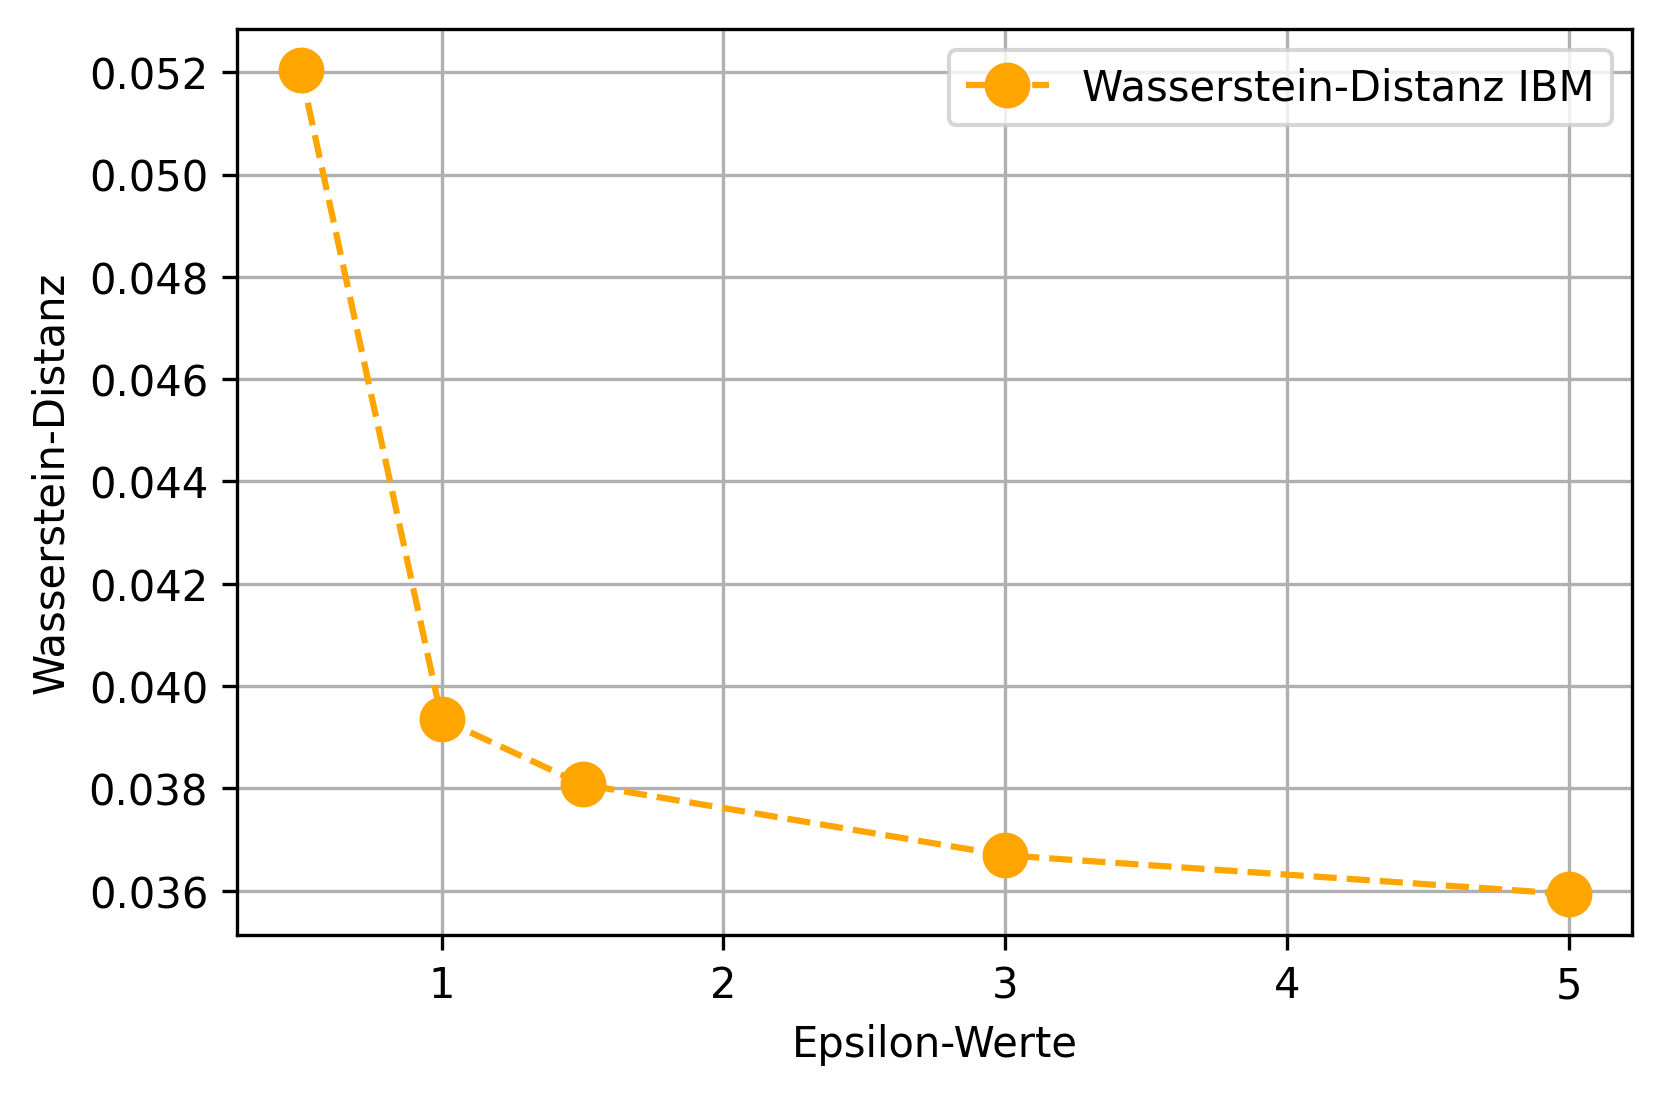
\includegraphics[scale=0.4]{./images/ibm_wsd.png}
	} \qquad
	\subfloat[Das Ergebnis von Google für die Wasserstein-Distanz.]{
		\label {fig:google_wsd}
		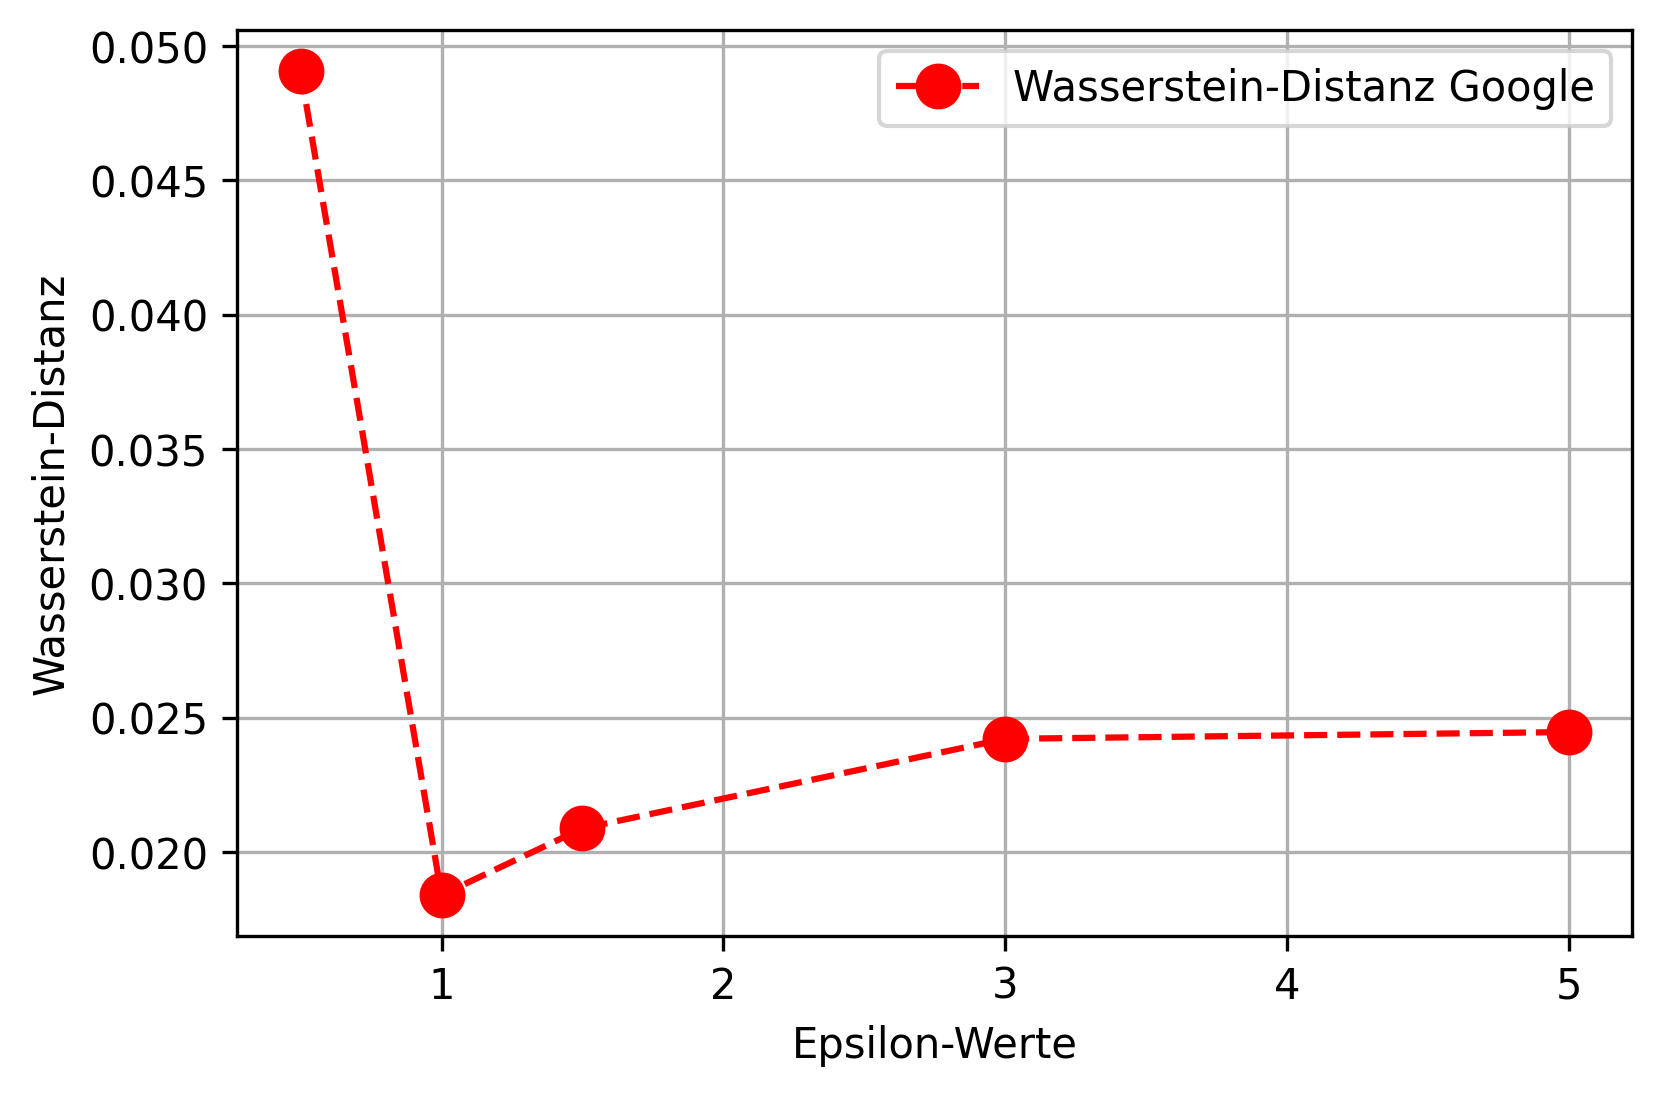
\includegraphics[scale=0.4]{./images/google_wsd.png}
	}
	\subfloat[Das Ergebnis von Smartnoise SDK für die Wasserstein-Distanz.]{
		\label {fig:sn_wsd}
		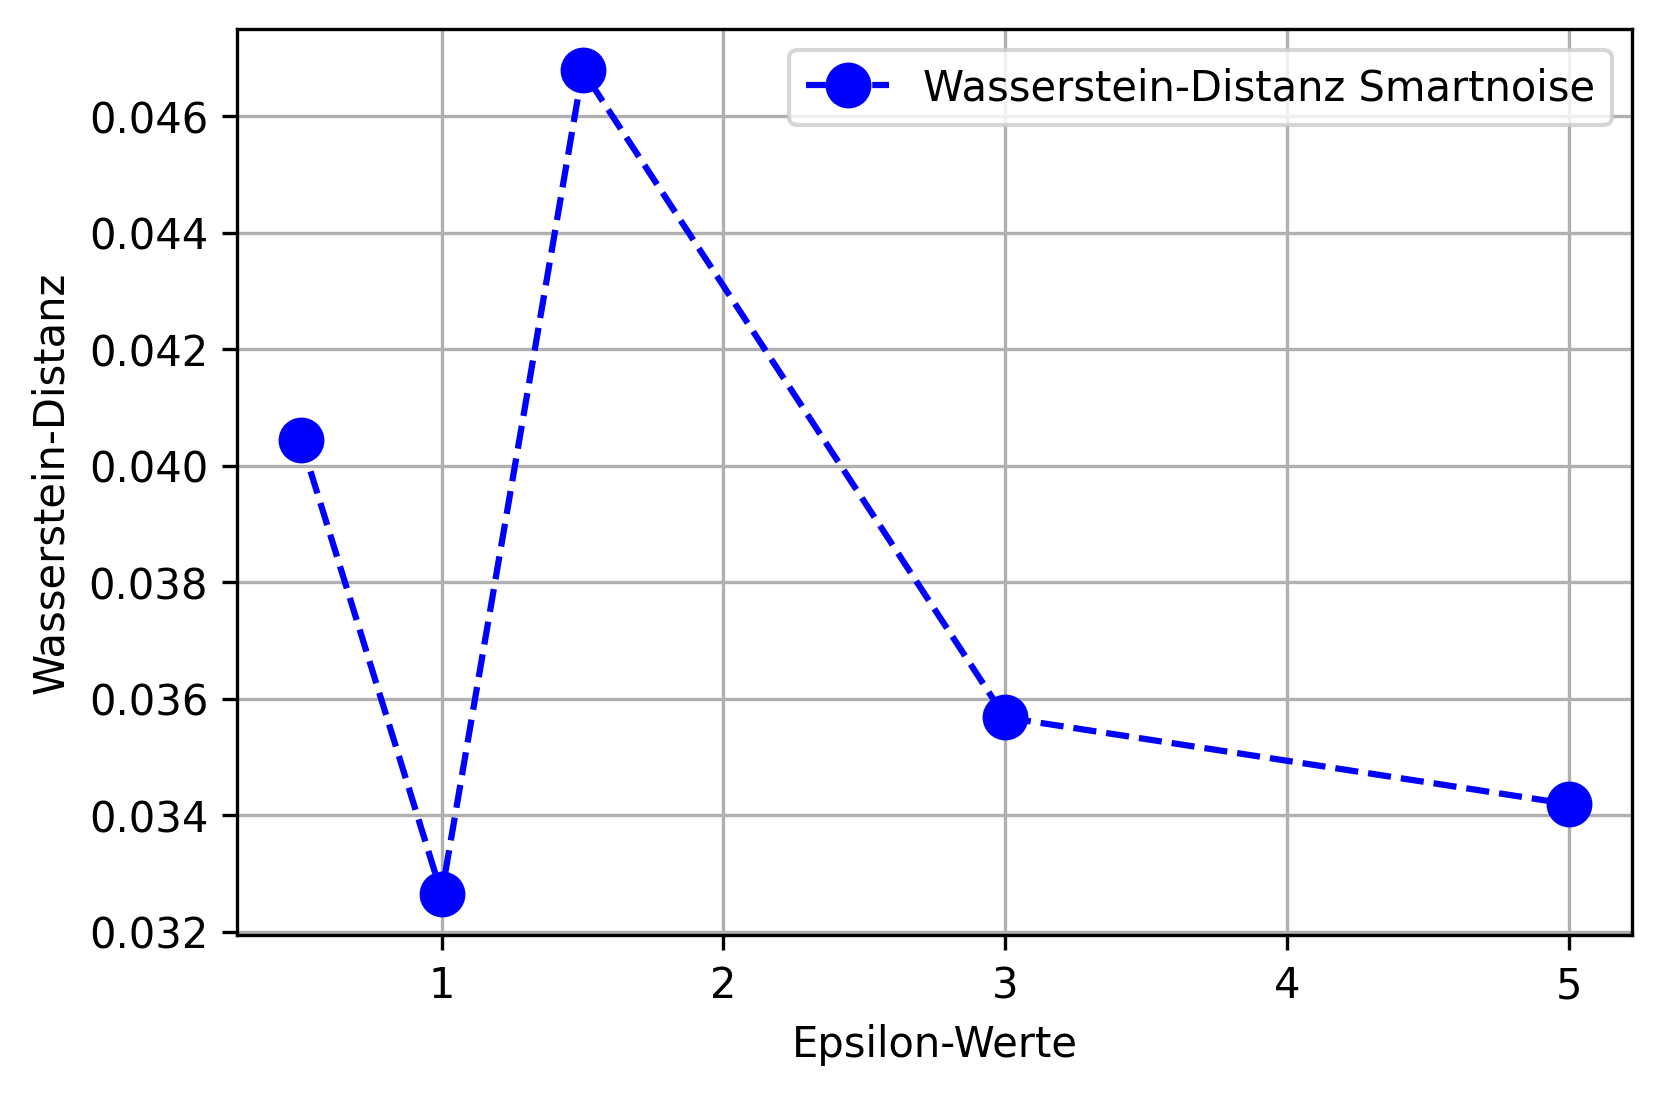
\includegraphics[scale=0.4]{./images/sn_wsd.png}
	}
	\caption{Die Ergebnisse der Wasserstein-Distanz für die $\epsilon$-Werte [0,5;1,0;1,5;3,0;5,0] der drei Frameworks.}
	\label{fig:wsd}
\end{figure}


\textbf{IBM \gls{dp} Ergebnis:}
Das Ergebnis entsprach den Erwartungen. In der \cref{fig:ibm_wsd} wird eine streng monoton fallende Kurve ersichtlich. Sie hat den Höchstwert der Wasserstein Distanz für den kleinsten $\epsilon$-Wert und das Minimum für den größten $\epsilon$-Wert. Die Differenz zwischen ihnen liegt bei ca. 0,015, sodass die Privatsphäre in einem relativ großem Wertebereich geschützt wird. Die Abnahme der Distanz erfolgt in Relation zum $\epsilon$-Wert gleichmäßig. Ab dem $\epsilon$-Wert 3,0 konvergiert der Wert der Distanz gegen ca. 0,0370. Daraus folgt ein Mindestwert der Wasserstein-Distanz für die Daten, somit ein Mindestniveau für den Schutz der Privatsphäre.

\textbf{Google Ergebnis:}
Das Ergebnis in \cref{fig:google_wsd} entsprach nicht einer streng monoton fallenden Kurve. Beim kleinsten $\epsilon$-Wert erreicht es einen hohen Wert. Dies stimmt noch mit der Erwartung überein. Anschließend folgen zwei Ausreißer für die $\epsilon$-Werte 1,0 und 1,5. Hierbei ist die Metrik deutlich niedriger als der vorherige Punkt ausgefallen. Die Differenz zwischen dem ersten und dem zweiten Punkt liegt bei ca. 0,03. Im weiteren Verlauf der Kurve bei dem $\epsilon$-Werten 3,0 und 5,0 steigt sie leicht an und konvergiert gegen einen Wert von ca. 0,0248. Die durchschnittliche Wasserstein-Distanz von 0,029 liegt nahe an diesem.

Die Privatsphäre wird für den kleinsten $\epsilon$-Wert sorgfältig geschützt, anschließend findet ein rapider Abfall des Schutzniveaus statt. Dies birgt gewisse Unsicherheiten bei kleinen $\epsilon$-Werten, bei denen hauptsächlich der Fokus auf der Privatsphäre liegt und diese vermehrt eingehalten werden müsste.

Die Ausreißer lassen sich anhand der Zwischenergebnisse erklären. Die Differenz der $\epsilon$-Werte 1,0 und 1,5 sind bei den verrauschten Datensätzen gering, somit liegen sie nah beieinander. Das Verrauschen der Durchschnitte fiel somit bei diesen $\epsilon$-Werten geringer aus, als beim $\epsilon$-Wert 0,5. Hierbei war die Differenz beim Zwischenergebnis viel höher, ein deutliches Verrauschen geht hieraus hervor. Durch diese Zwischenergebnisse ist festgestellt, dass das unerwartete Verhalten der Kurve auf das Framework zurückzuführen ist. 
In diesem Framework folgen verschiedene Berechnungen für den Laplace Mechanismus, welcher für das Verrauschen verantwortlich ist, die als außenstehender nicht verständlich sind. Daher ist das Ergebnis teils unerklärbar, da die Zuweisung des Verrauschens auf die Rohdaten vom Framework ausgeht.

\textbf{Smartnoise SDK Ergebnis:}
Die ersten drei Punkte der $\epsilon$-Werte widersprechen den Erwartungen wie in \cref{fig:sn_wsd} ersichtlich. Der erste Punkt ist nicht der Höchstpunkt der Kurve. Dieser liegt beim dritten Punkt mit 0,0468 vor. Der zweite Punkte ist der Tiefpunkt der Kurve, sodass die Privatsphäre hierbei sehr gering geschützt ist. Ab dem dritten Punkt ist der Verlauf streng monoton fallend und entspricht somit der Erwartung. Beim ersten Punkt liegt der Wert zwischen dem zweite und dritten, da die Differenz der Zwischenergebnisse im Verhältnis zu den anderen dazwischen liegt. Hier war das Verrauschen im Verhältnis zum zweiten Punkt deutlich mehr, jedoch zum dritten Punkt geringer.

Die Zwischenergebnisse spiegeln die unerwartete Verteilung der drei ersten Punkte in der Metrik wieder. Diese Werte sind für die beiden Datensätze am $\epsilon$-Wert 1 sehr nah beieinander, wofür das geringe Verrauschen des Frameworks verantwortlich ist. Daraus folgt der niedrige Schutz der Privatsphäre. Dagegen beim $\epsilon$-Wert 1,5 ist die Differenz zwischen den Zwischenergebnissen höher als zuvor, wodurch die Metrik ein hohen Wert hat. Dieses Verhalten ist auf die den Laplace Mechanismus im Framework zuzuweisen. Er agiert hier nicht entsprechend der Definition von \gls{dp}. Dies ist eine Implementierungsangelegenheit, die entscheidet wie stark das Verrauschen ist, die lediglich vom Nutzer angewendet und beurteilt werden kann.

\begin{figure}[htbp]
	\centering
	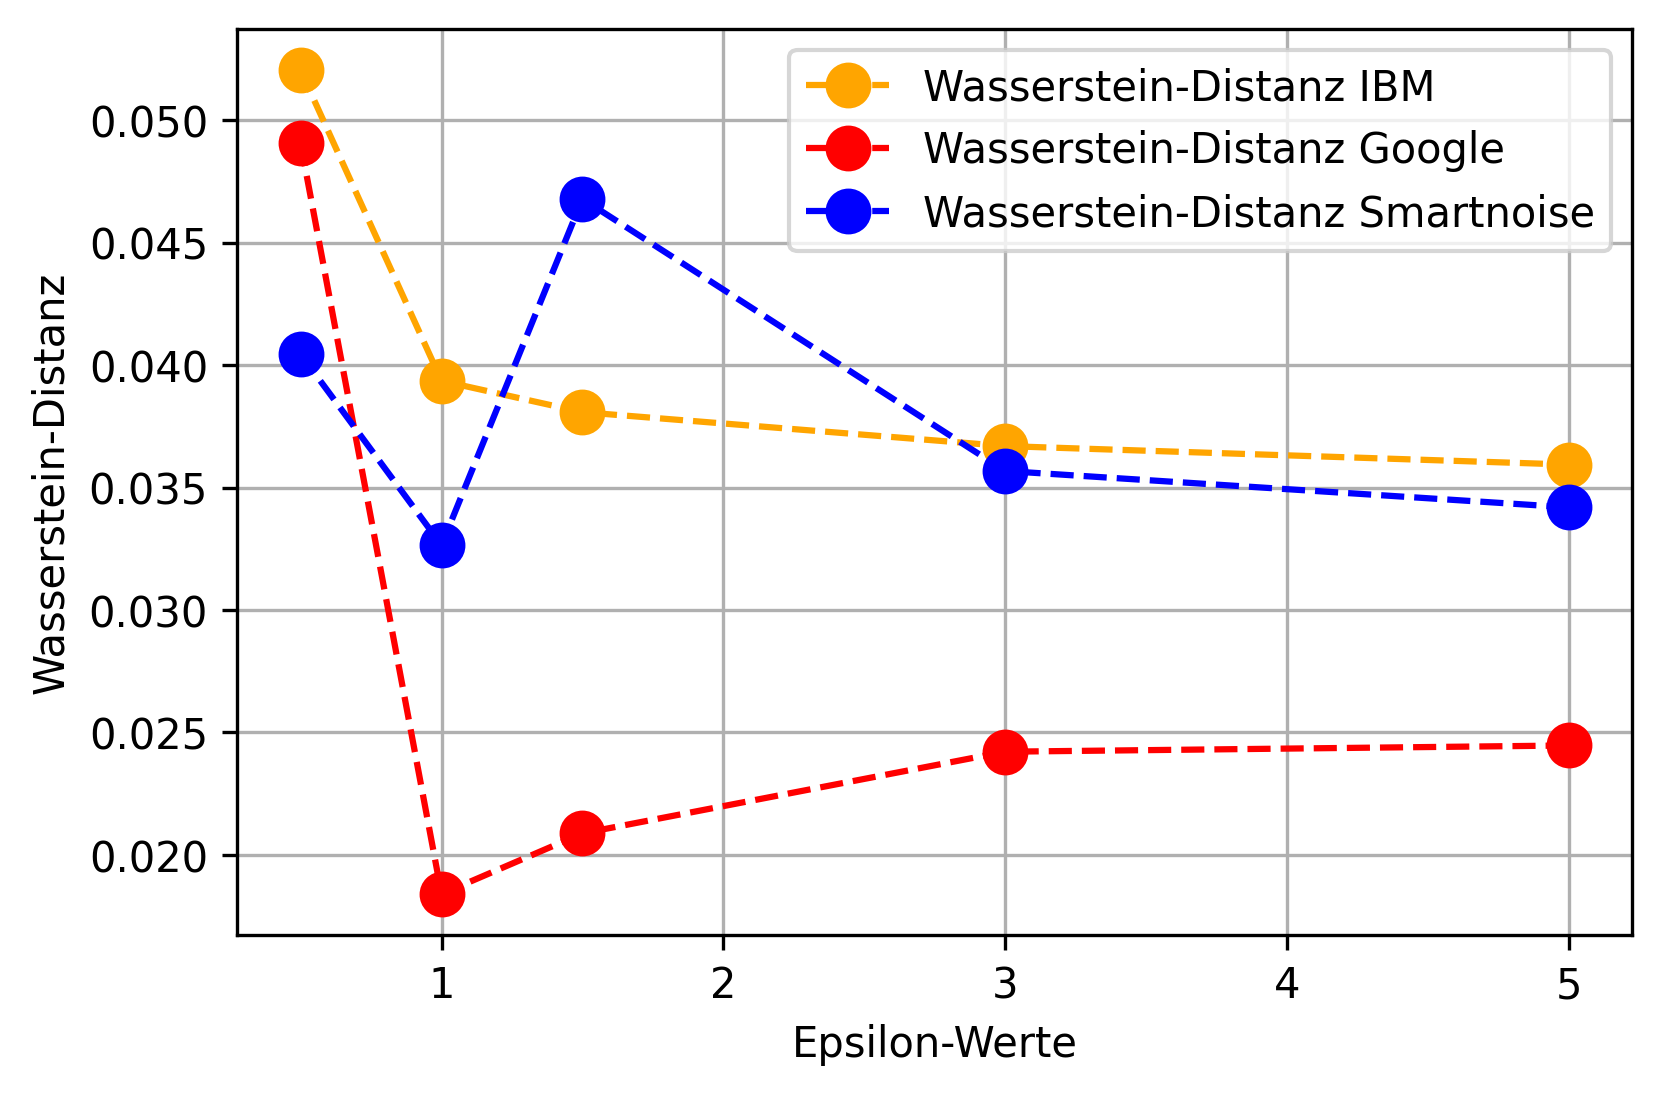
\includegraphics[scale=0.6]{./images/together_wsd.png}
	\caption{Die Gesamtübersicht der drei Frameworks in der Metrik Wasserstein-Distanz.}
	\label{fig:together_wsd}
\end{figure}

\textbf{Vergleich: }
In \cref{fig:wsd} werden die Ergebnisse der drei Frameworks in Vergleich gesetzt. Beim ersten $\epsilon$-Wert liegt bei jedem Framework außer beim Smartnoise SDK der Höchstwert vor. Ab diesem Punkt fällt der Wert der restlichen Punkte bei Google \gls{dp} in Gegensatz zu den anderen erheblich ab. Sie verläuft ohne eine Überschneidung unterhalb der anderen Frameworks zu haben. Die Kurve von IBM \gls{dp} hat insgesamt den Höchstwert und verläuft von diesem streng monoton fallend weiter. Sie behält bis zum $\epsilon$-Wert 5 stets den höchsten Wert für die Metrik außer beim $\epsilon$-Wert 1.5, hier liegt das Ergebnis von Smartnoise SDK höher. Ab dem vierten Punkt verlaufen die Ergebnisse dieser zwei Frameworks (IBM \gls{dp} und Smartnoise SDK) sehr nah beieinander, was für eine Konvergenz des Schutzes für die Privatsphäre bedeutet. Um ca. 0,01 liegt parallel dazu die Ergebnisse von Google vor. Insgesamt verlaufen die Kurven von IBM \gls{dp} und Smartnoise SDK im mittlerer oberer Bereich in Gegensatz zu Google im unteren.

Die Privatsphäre wird unterschiedlich stark bei den Frameworks geschützt. Beim IBM \gls{dp} ist ein stets hohes Niveau an Privatsphäre vorhanden. Dieser konvergiert ebenfalls auf einem hohen Niveau für große $\epsilon$-Werte. Somit ist ein hoher Schutz der Rohdaten vorhanden. Dagegen beim Google \gls{dp} fällt das Niveau des Schutz nach dem ersten Punkt erheblich. Vor allem bei kleinen $\epsilon$-Werten kann das Framework nicht einen hohen Schutz an Privatsphäre aufrechterhalten und hat in diesen den geringsten Schutz an Privatsphäre. Im Nachgang konvergiert es für weitere steigende $\epsilon$-Werte, jedoch auf dem niedrigsten Niveau in Verhältnis zu den restlichen Frameworks. Smartnoise SDK zeigt ein Verhalten auf, welches zwischen den beiden anderen liegt. Zum einen geht eine Instabilität bei den ersten drei Punkten hervor, die trotz dessen ein hohen Schutz an Privatsphäre anbieten. Zum anderen liegt die Konvergenz des Frameworks fast auf dem selben des IBM \gls{dp}, welches in bei kleinen $\epsilon$-Werten besser abschneidet.
\newpage
\section{Genauigkeit}
In diesem Abschnitt werden die Ergebnisse auf ihre Genauigkeit des Wertes zum unveränderten Datensatz beurteilt. Zu einem gibt die mittlere quadratische Abweichung ein Einblick auf die Auswirkung des Verrauschens. Zum anderen verschafft die Standardabweichung die Erkenntnis, inwieweit die Mechanismen stabil die Werte im Verhältnis zu den $\epsilon$-Werten Verrauschen. 

\subsection{Mittlere quadratische Abweichung}
Bei der mittleren quadratischen Abweichung war die Eingabe der erste verrauschte und der unveränderte Datensatz. Der Wert zeigt eine Tendenz des Frameworks auf, ob das Verrauschen verstärkt oder vermindert eingesetzt wird.

\textbf{Erwartetes Ergebnis:}
Desto größer die mittlere quadratische Abweichung ist, desto ungenauer sind die verrauschten Daten. Der umgekehrte Fall gilt ebenfalls. Das Ergebnis soll mit steigendem $\epsilon$-Wert genauer werden.
\begin{figure}[htbp]
	\centering
	\subfloat[Das Ergebnis von IBM \gls{dp} für die mittlere quadratische Abweichung.]{
		\label {fig:ibm_mse}
		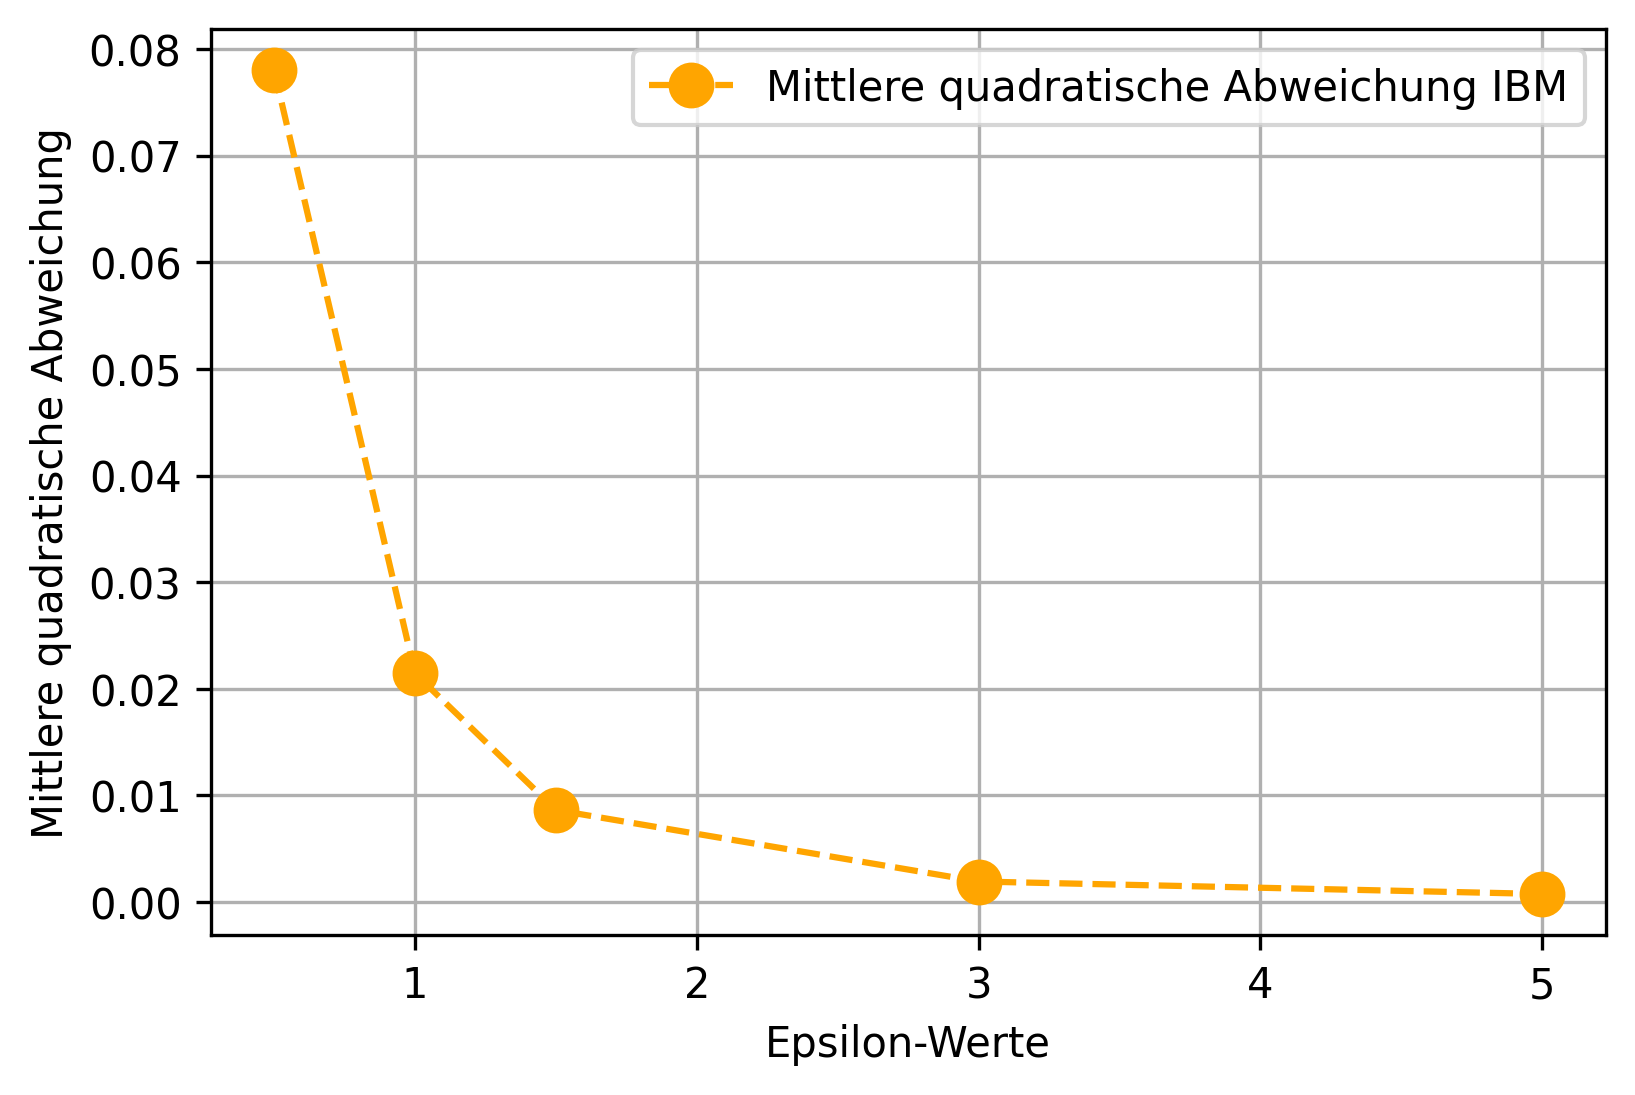
\includegraphics[scale=0.4]{./images/ibm_mse.png}
	} \qquad
	\subfloat[Das Ergebnis von Google für die mittlere quadratische Abweichung.]{
		\label {fig:google_mse}
		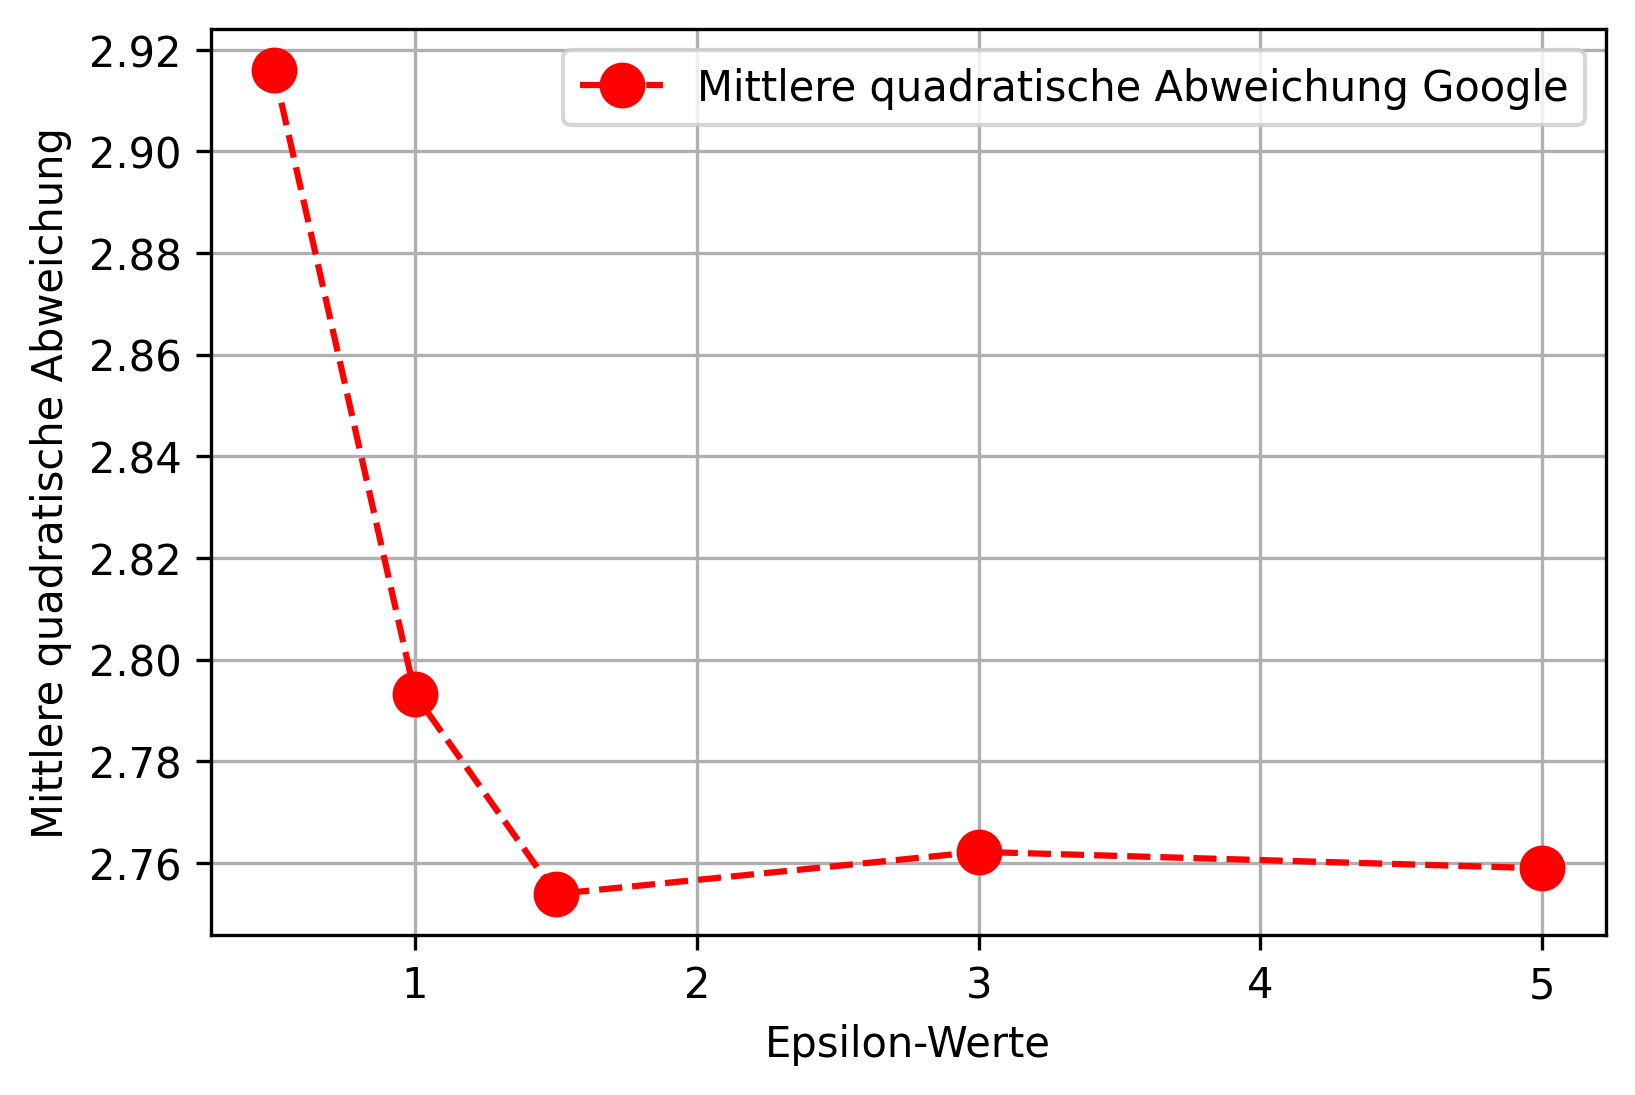
\includegraphics[scale=0.4]{./images/google_mse.png}
	}
	\subfloat[Das Ergebnis von Smartnoise SDK für die mittlere quadratische Abweichung.]{
		\label {fig:sn_mse}
		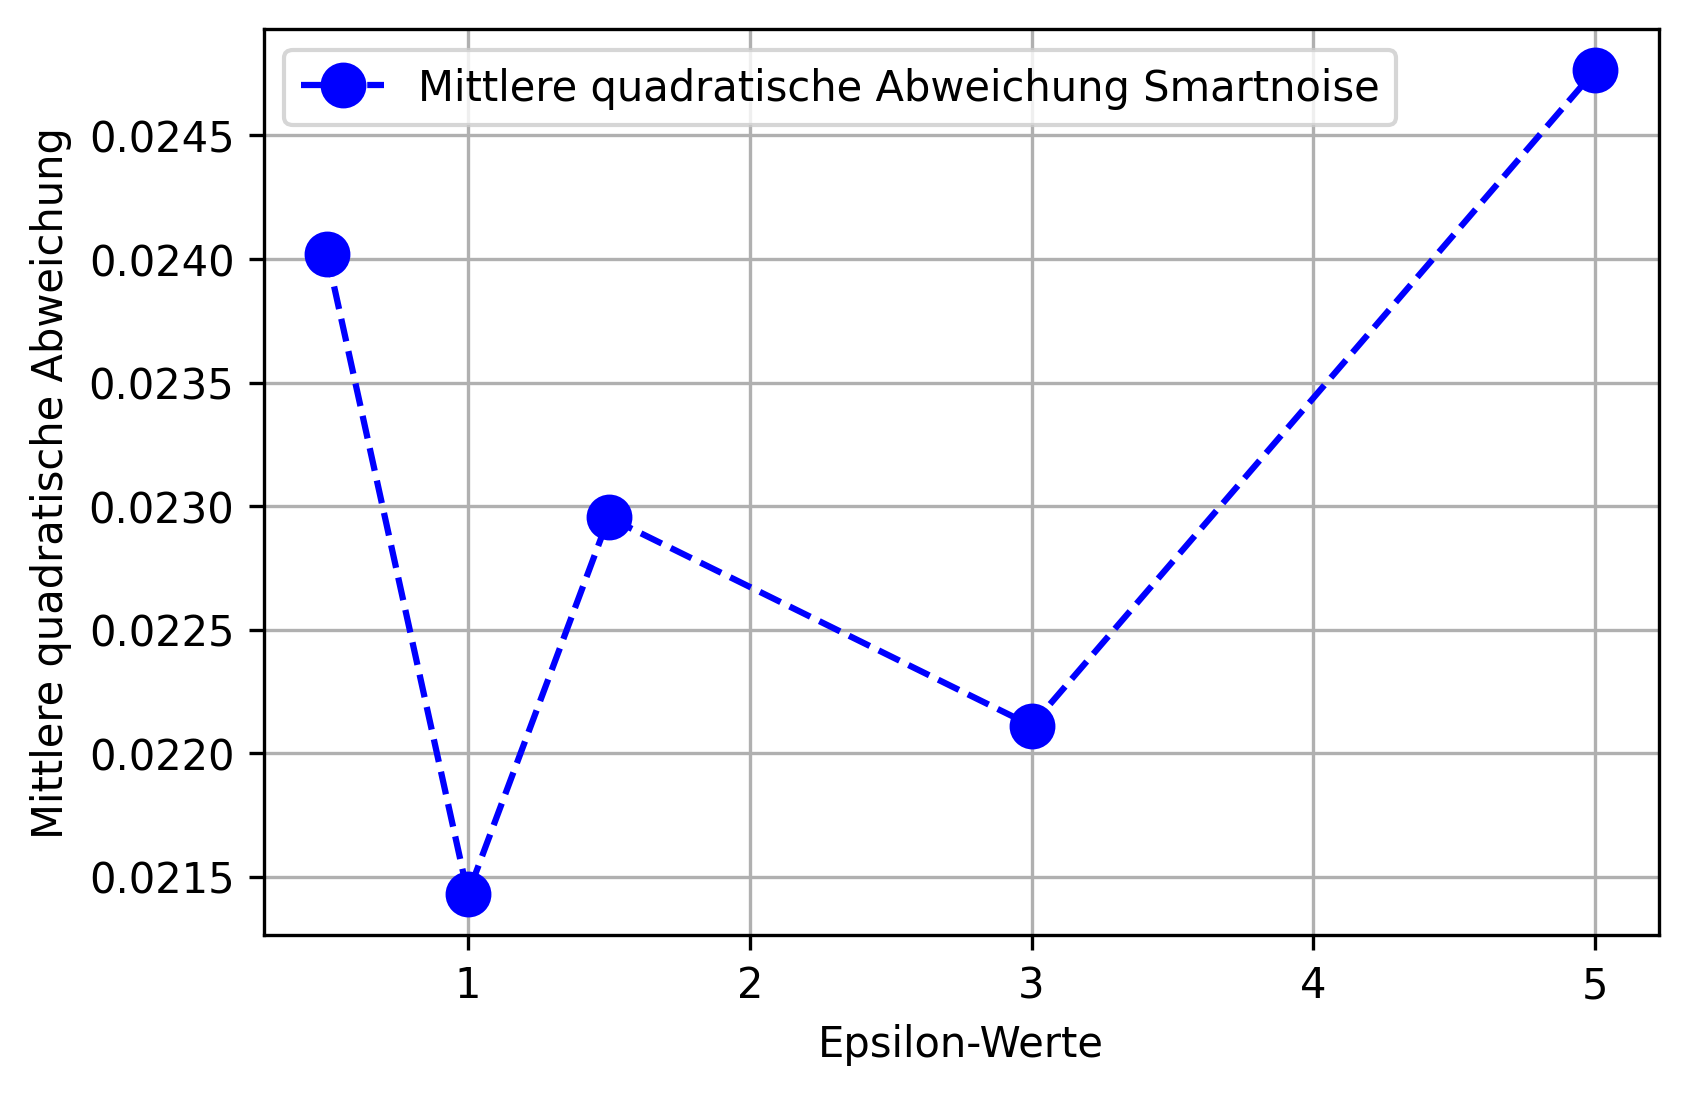
\includegraphics[scale=0.4]{./images/sn_mse.png}
	}
	\caption{Die Ergebnisse der mittleren quadratischen Abweichung der drei Frameworks für die $\epsilon$-Werte [0,5;1,0;1,5;3,0;5,0].}
	\label{fig:mse}
\end{figure}

\textbf{IBM \gls{dp} Ergebnis:}
Die Genauigkeit nimmt mit steigendem $\epsilon$-Wert zu, die fallende Kurve entspricht der Erwartung wie in \cref{fig:ibm_mse} ersichtlich. Ein Gesamtblick auf die Werte der Metrik zeigt eine hohe Genauigkeit auf. Vom ersten bis zum letzten Punkt steigt die Genauigkeit fast um das achtfache. Schon beim zweiten Punkt ist die Genauigkeit sehr gestiegen und der verrauschte Durchschnitt des Frameworks übereinstimmt fast mit dem des unveränderten beim fünften Punkt.

In den Zwischenergebnissen wird diese Auswertung deutlich, da diese sich nur in den Nachkommastellen zum originalen Durchschnittswert 36,1 variieren. Somit kann eine hohe Genauigkeit beobachtet werden.

\textbf{Google Ergebnis:}
Das Ergebnis in \cref{fig:google_mse} entspricht bis auf den 4 Punkt der Erwartung. Die Kurve hat ihren Höchstpunkt beim $\epsilon$-Wert 0,5 und sinkt mit steigendem $\epsilon$-Wert. Die weiteren Punkt nehmen einen niedrigeren Wert für die Abweichung an. Beim vierten Punkt ist der Wert minimal höher als der vorherige und nachherige, wodurch die strenge Monotonie unterbrochen wird. Ebenfalls ist ab diesem Punkt eine Konvergenz ersichtlich, sodass für weitere höhere $\epsilon$-Werte diese Metrik um den Wert 2.76 betragen würde.

Der unveränderte Durchschnitt beträgt 36.1 und in den Zwischenergebnisse hat der verrauschten Durchschnitt ca. den Wert 34. Er ist stets niedriger und nimmt mit steigendem $\epsilon$-Wert wie erwartet nicht zu. Dies weist ein internes Verhalten auf, welches als negatives Rauschen in den Zwischenergebnissen zum Vorschein kommt. Dies erklärt den hohen Wert für die mittlere quadratische Abweichung, wodurch eine hohe Ungenauigkeit vorliegt. Die verrauschten Werte haben eine weite Entfernung zu den originalen, welche sogar für große $\epsilon$-Werte nicht abnimmt, sondern stagniert. Diese weite Distanz ist vom Laplace Mechanismus vorgegeben, die unveränderbar ist. Das Framework berechnet das Hinzufügen des Rauschens nach seinen eigenen Vorgaben, sodass dieses Phänomen nachzuvollziehen erfordert eine tiefstgehende Untersuchung, was nicht Bestandteil dieser Bachelorarbeit ist und es in der Ausgabe fest vorhanden ist.

\textbf{Smartnoise SDK Ergebnis:}
Das Ergebnis in \cref{fig:sn_mse} besitzt am zweiten sowie fünften Punkt einen Ausreißer. Der Höchstpunkt liegt nicht am ersten sondern am fünften, sodass die höchste Ungenauigkeit beim größten anstatt am kleinsten $\epsilon$-Wert vorliegt. Beim zweiten Punkt handelt es sich um den Tiefstpunkt der Ungenauigkeit, welcher beim fünften liegen sollte. Da sonst am zweiten Punkt, bei einem kleinen $\epsilon$-Wert eine höhere Genauigkeit als an den anderen Punkten zutrifft.

In den Zwischenergebnissen liegen die verrauschten Durchschnitte um den originalen Durchschnittswert 36.1, weswegen die Werte der Metrik gering ausgefallen sind. Des Weiteren verursacht die randomisierte Zuweisung des Verrauschens vom Laplace Mechanismus für die Ausreißer. Hierbei liegen die Zwischenergebnisse sehr nah beieinander, sodass die Unterschiede in den Nachkommastellen deutlich werden. Dies kann der Grund für die fehlende strenge Monotonie sein. Kleine Abweichungen in ihnen verursachen große Schwankungen in den Metriken, welche stärker als bei unterschiedlichen $\epsilon$-Werten. Insgesamt sorgt das Framework für eine sehr hohe Genauigkeit für kleine sowie große $\epsilon$-Werte. Ein erheblicher erwartete Unterschied zwischen den verschiedenen $\epsilon$-Werten ist nicht erkenntlich.
\begin{figure}[!htbp]
	\centering
	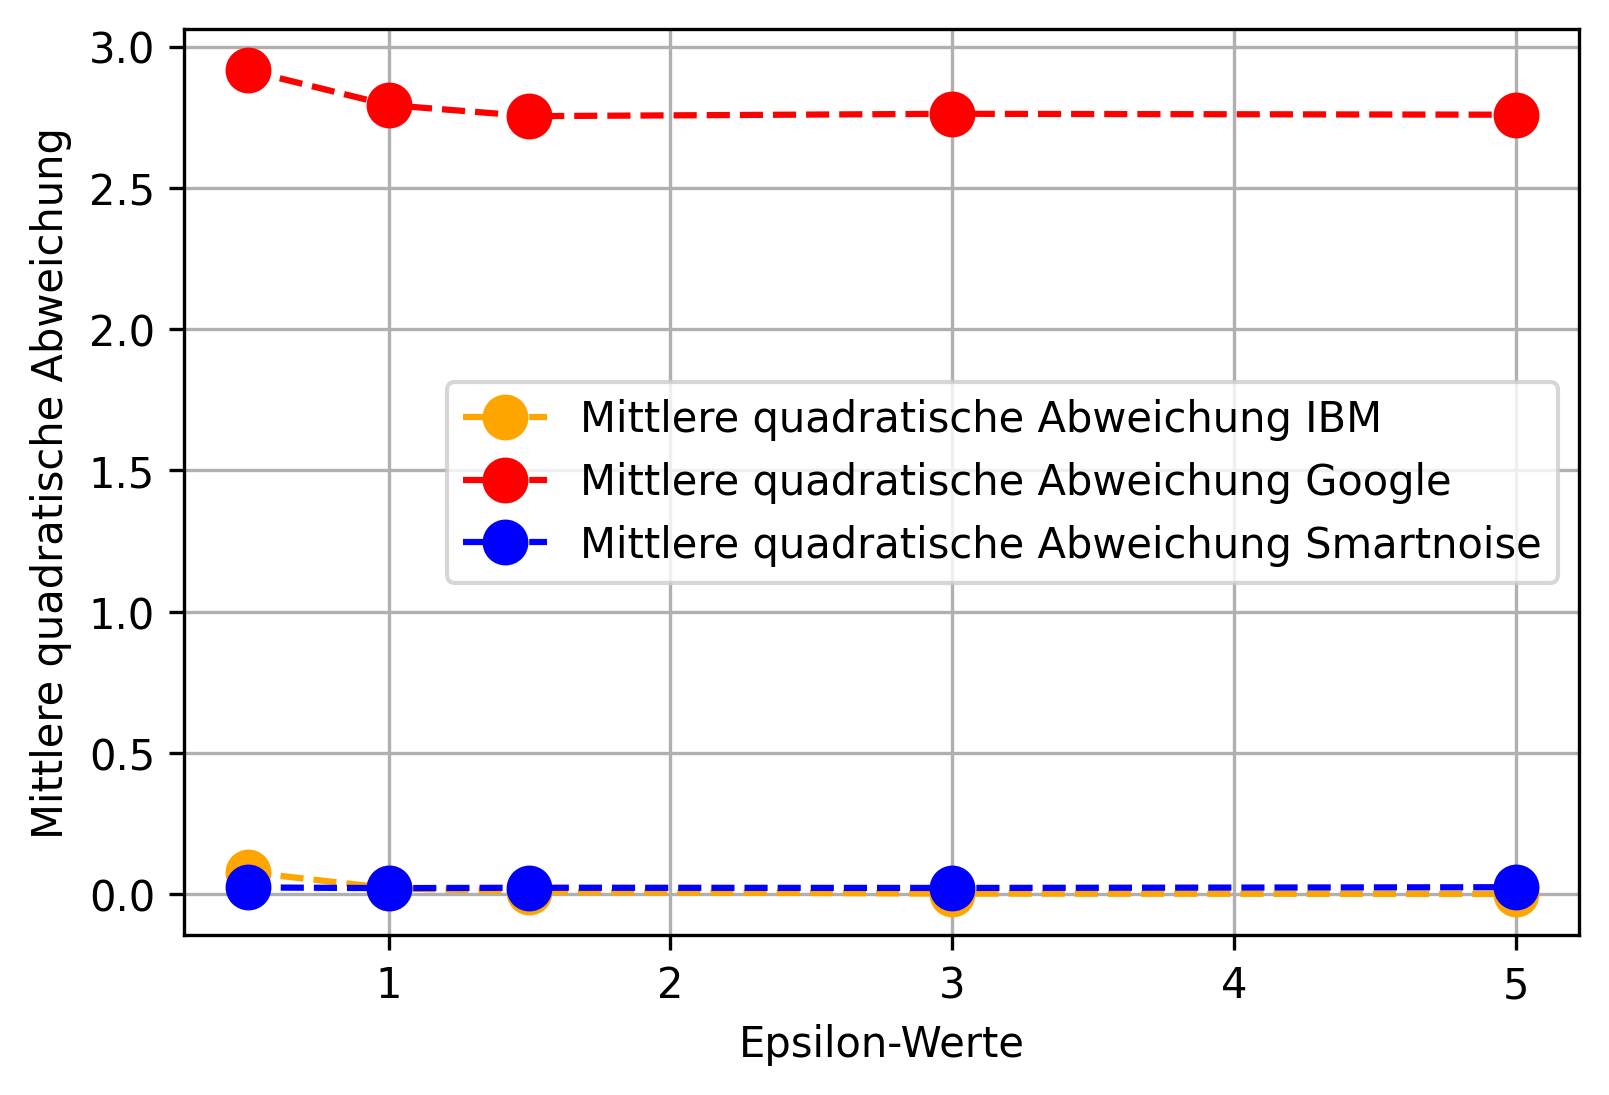
\includegraphics[scale=0.6]{./images/together_mse.png}
	\caption{Die Gesamtübersicht der drei Frameworks in der Metrik Mittlere quadratische Abweichung.}
	\label{fig:together_mse}
\end{figure}

\textbf{Vergleich: }
Im Gesamtüberblick in \cref{fig:together_mse} wird der Grad der Genauigkeit der Frameworks eindeutig erkennbar. IBM \gls{dp} und Smartnoise SDK befinden sich nahe des Wertes $0$ für die Metrik. Aus dieser Perspektive ist keine erkenntliche Unterscheidung zwischen kleinen und großen $\epsilon$-Werten in der Genauigkeit sichtbar. Daher ist die Beurteilung von IBM \gls{dp} und Smartnoise SDK in der zu vorigen spezifischen Beschreibungen eindeutig. Hier kann das Verhältnis zu einander analysiert werden.
Die Kurve von Google sticht zu den anderen deutlich hervor. Sie ist wie die beiden von IBM \gls{dp} und Smartnoise SDK im Gesamten konstant und verläuft um den Wert 3. Dieser weist auf eine durchgehende hohe Ungenauigkeit der verrauschten Daten hin. In Relation zu den anderen sorgt das Verrauschen vom Google Laplace Mechanismus für einen zu niedrigen Wert. Sein Rauschen ist im Allgemeinen zu stark.

\subsection{Standardabweichung}
Anhand der Standardabweichung wird die Stabilität der Genauigkeit des Laplace Mechanismus bestimmt. Dafür ist lediglich der erste verrauschte Datensatz als Eingabe notwendig.

\textbf{Erwartetes Ergebnis:}
Die Abweichung der Werte um den Mittelwert weißt auf die Sorgfalt des Mechanismus hin. Wenn eine große Abweichung bei kleinen $\epsilon$-Werten vorliegt, dann ist die Privatsphäre besser geschützt, jedoch nimmt die Stabilität der Genauigkeit ab. Die höhere Abweichung sorgt für verschiedene verrauschte Werte, die damit insgesamt ihre Genauigkeit senkt. Im umgekehrten Fall gilt dies ebenfalls. Vor allem bei großen $\epsilon$-Werten ist eine hohe Stabilität in der Genauigkeit zu erwarten, da dann der Mechanismus weniger Rauschen dazu addiert.

\begin{figure}[htbp]
	\centering
	\subfloat[Das Ergebnis von IBM \gls{dp} für die Standardabweichung.]{
		\label {fig:ibm_std}
		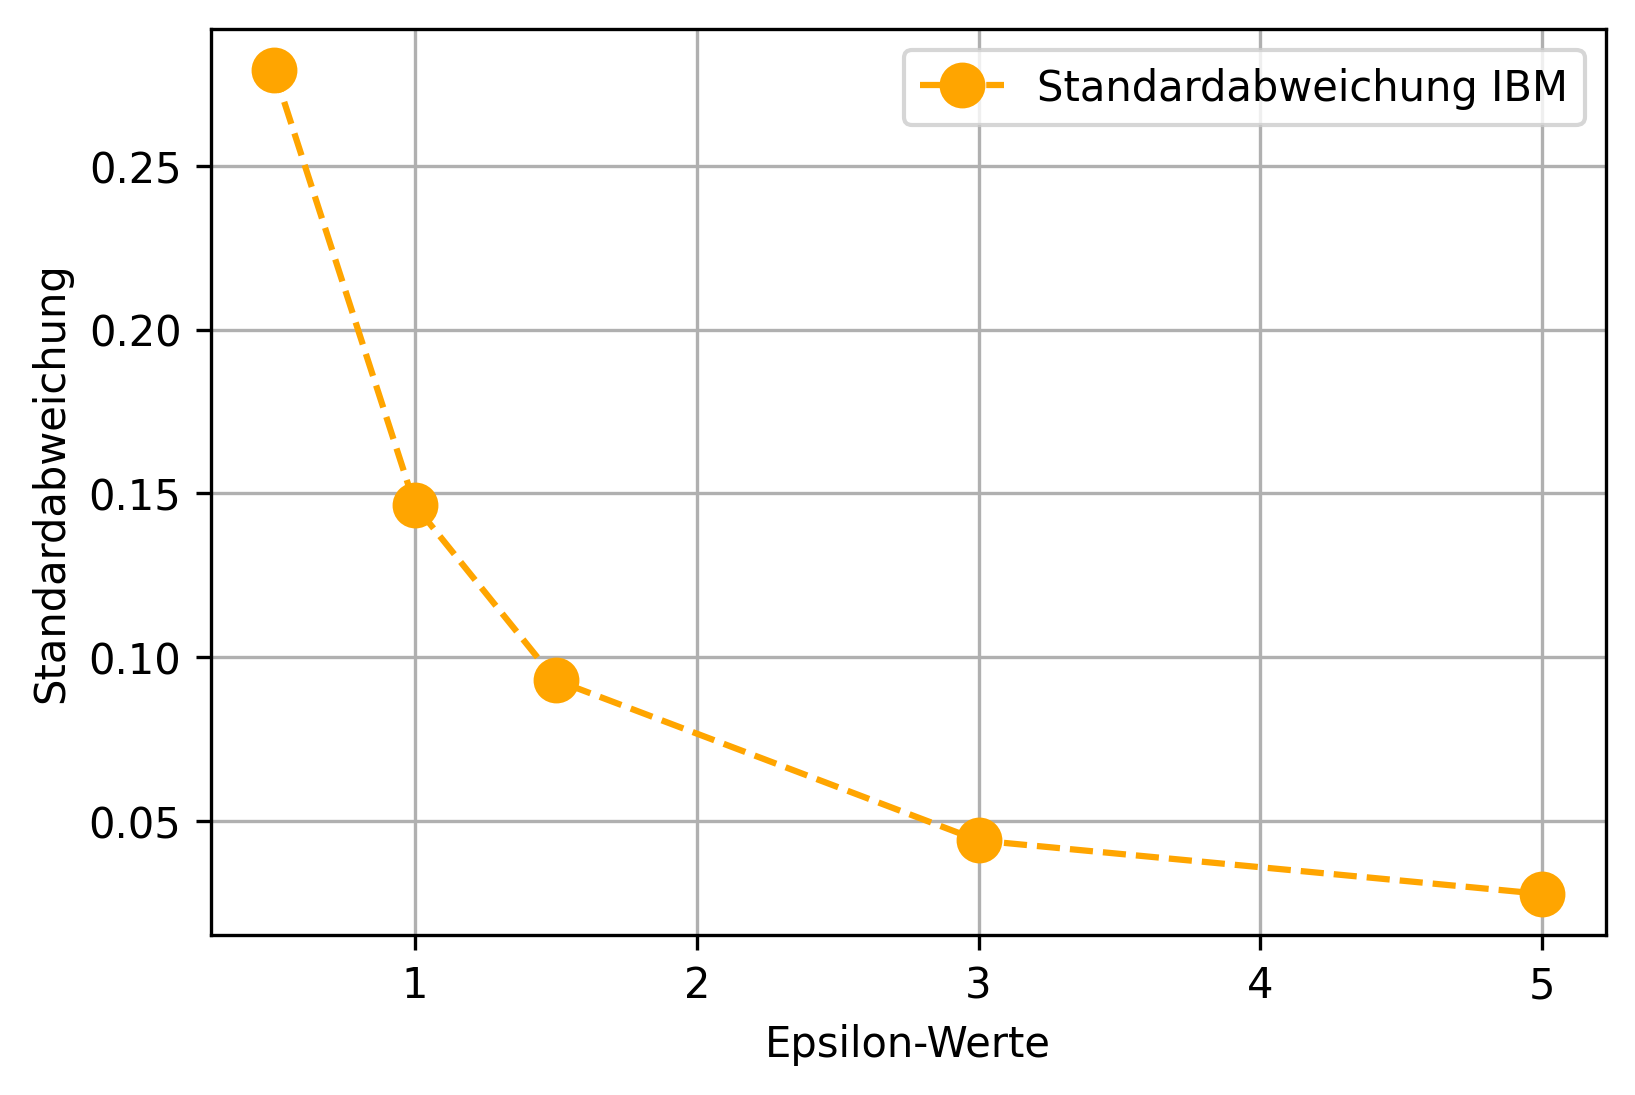
\includegraphics[scale=0.4]{./images/ibm_std.png}
	} \qquad
	\subfloat[Das Ergebnis von Google für die Standardabweichung.]{
		\label {fig:google_std}
		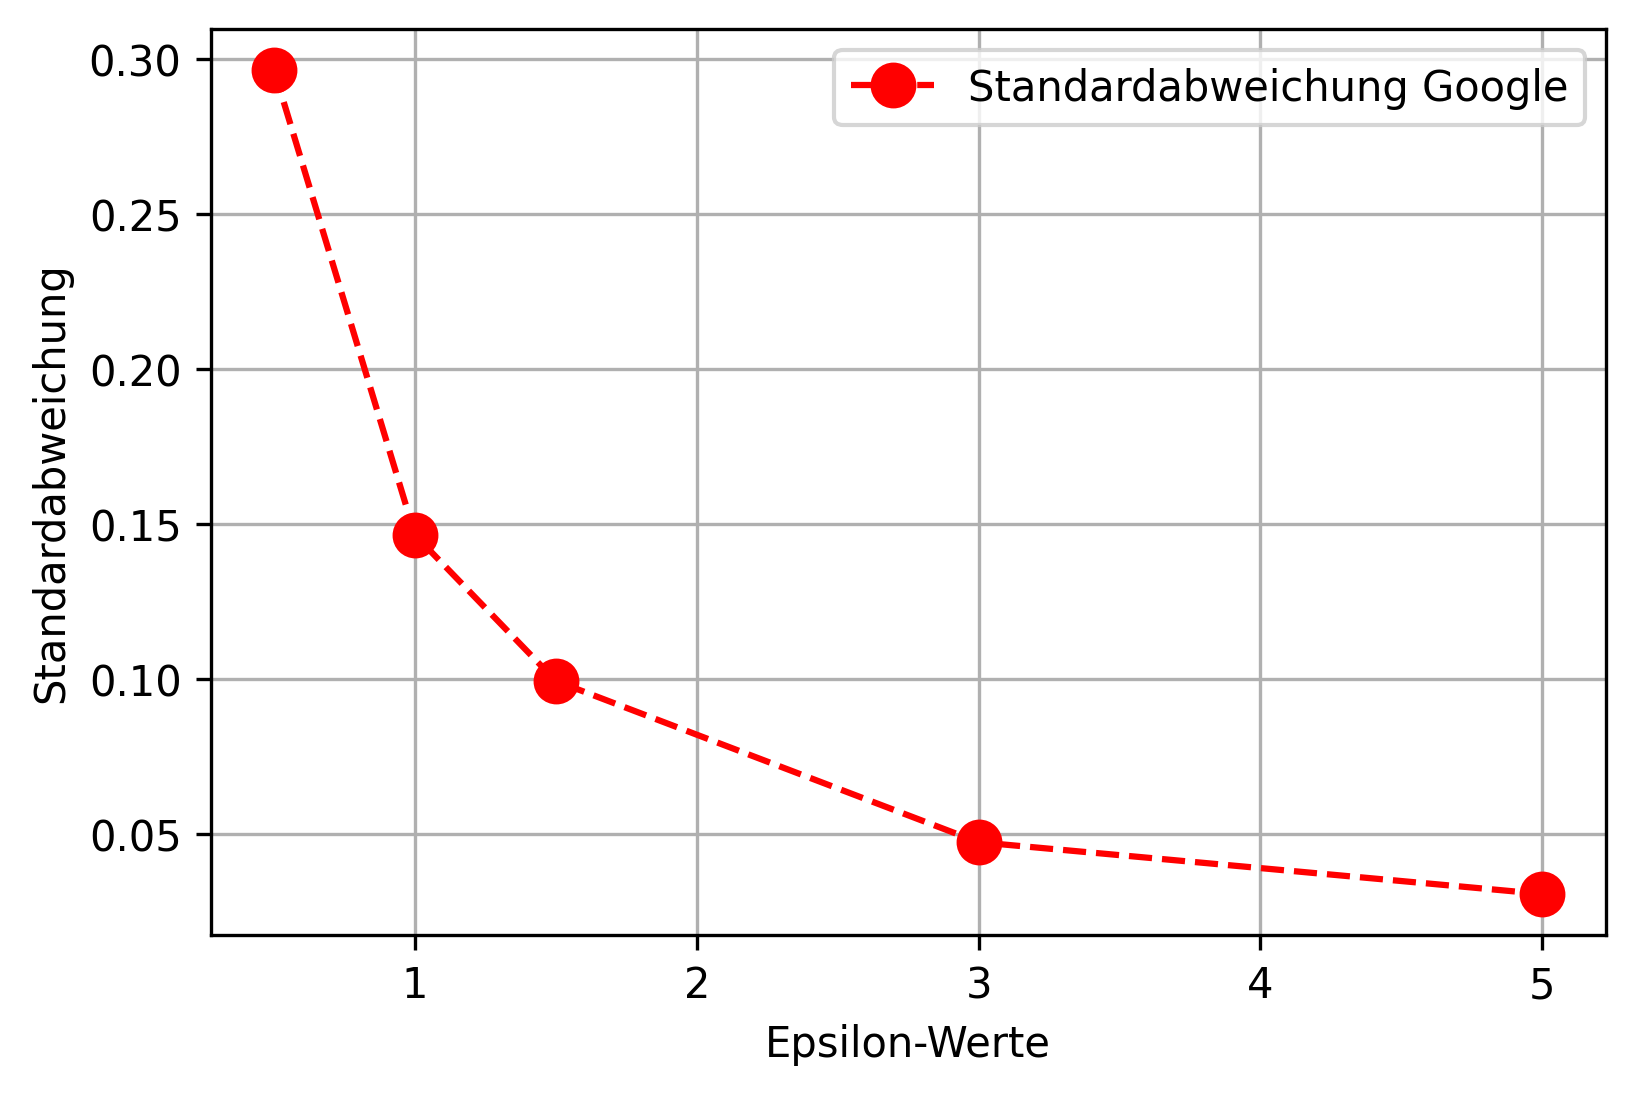
\includegraphics[scale=0.4]{./images/google_std.png}
	}
	\subfloat[Das Ergebnis von Smartnoise SDK für die Standardabweichung.]{
		\label {fig:sn_std}
		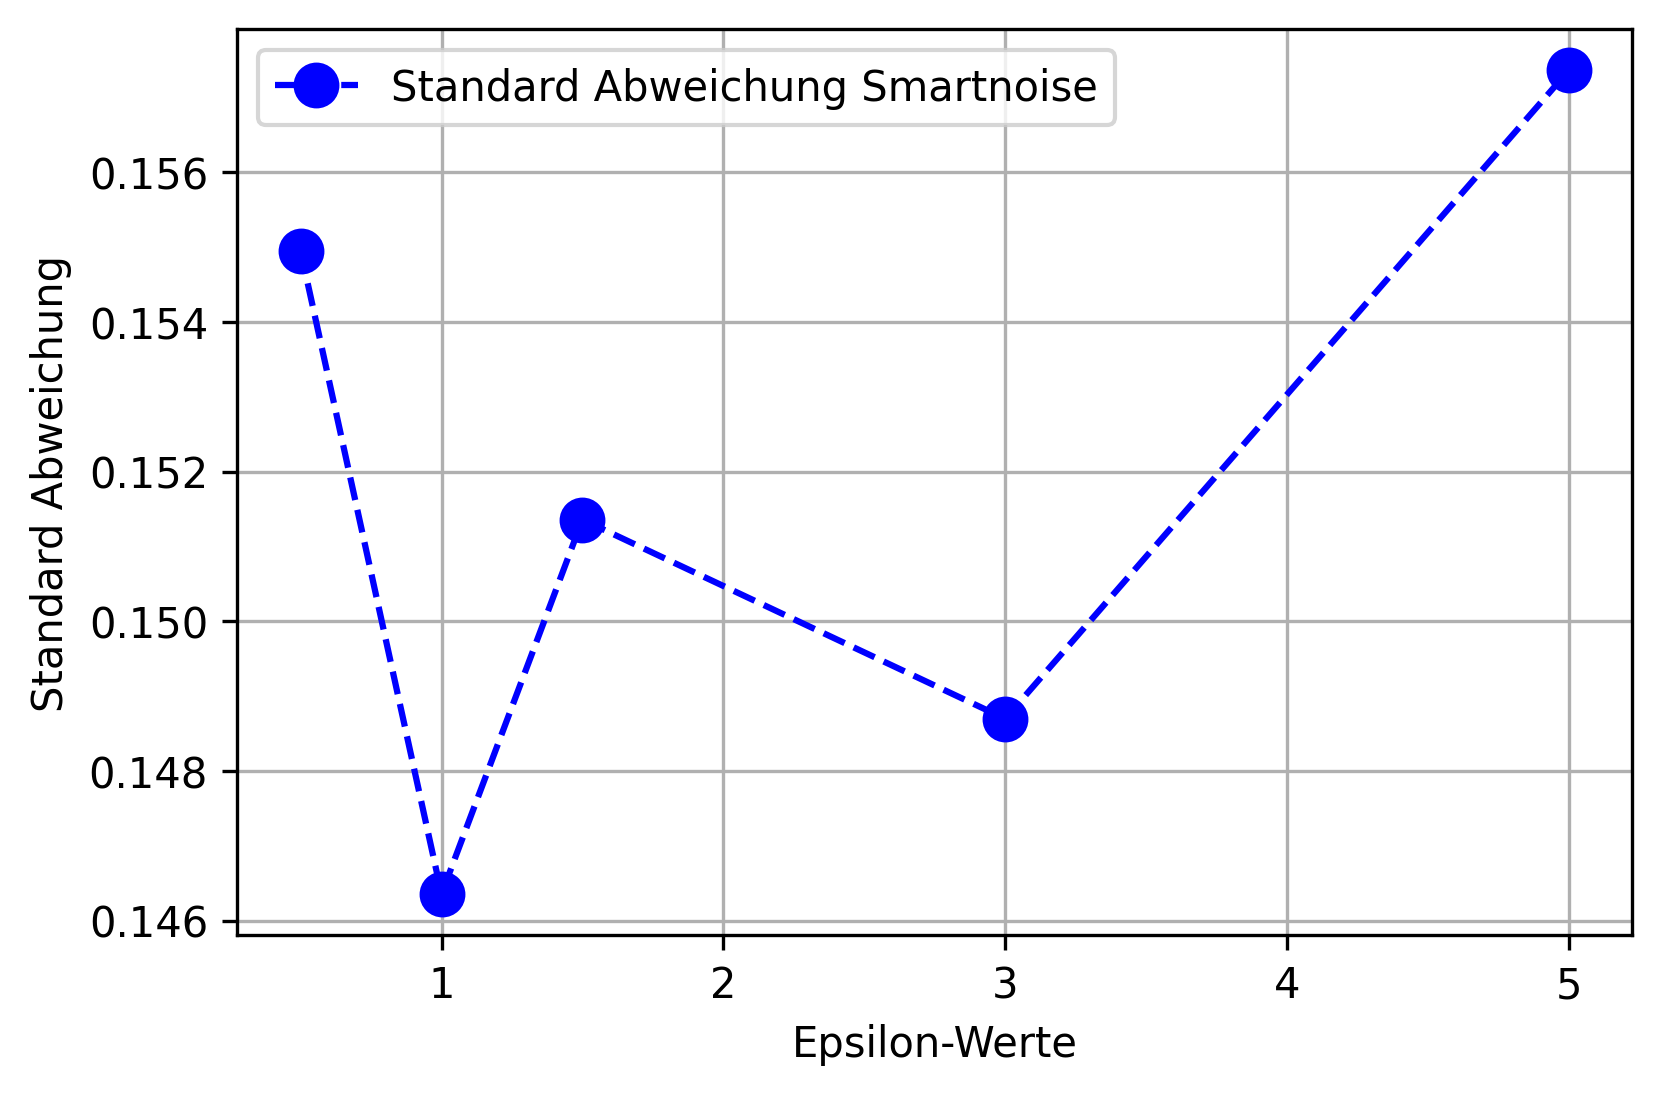
\includegraphics[scale=0.4]{./images/sn_std.png}
	}
	\caption{Die Ergebnisse der Standardabweichung für die $\epsilon$-Werte [0,5;1,0;1,5;3,0;5,0] der drei Frameworks.}
	\label{fig:std}
\end{figure}

\textbf{IBM \gls{dp} Ergebnis:}
Bei diesem Ergebnis in \cref{fig:ibm_std} spricht die streng monoton fallende Kurve für eine zunehmende Stabilität bei steigendem $\epsilon$-Wert. Dieses Verhalten entspricht der Definition von \gls{dp}. Für einen kleinen $\epsilon$-Wert wird die Privatsphäre mehr geschützt und die Genauigkeit dafür vernachlässigt, daher sind die Ausgaben variierter.Dies spiegelt sich in den ersten drei Punkten wieder. Die letzten zwei Punkte sprechen für eine hohe Stabilität der verrauschten Daten, da der Wert sehr nahe bei $0$ liegt. Somit wird kaum noch die Werte stärker verrauscht.

\textbf{Google Ergebnis:}
Die Kurve erfolgt den Erwartungen streng monoton fallenden wie in \cref{fig:google_std} erkennbar zu sein. Bei kleinen $\epsilon$-Werten ist die Abweichung höher als bei größeren. Dies deutet auf eine größere Instabilität in der Ausgabe bei kleinen $\epsilon$-Werten. Der Wertebereich der Metrik nimmt um ein Sechstel ab, was eine hohe Präzision des Mechanismus aufzeigt. Er agiert bei kleinen sowie großen $\epsilon$-Werten stets richtig. Auffallend sind die letzten zwei Punkte, welche sehr nahe an $0$ liegen. Dafür wird vom Laplace Mechanismus nur Verrauschen in den Nachkommastellen hinzugefügt, welche nicht mehr signifikant die Werte ändern. In den Zwischenergebnissen wird dies deutlich, da sie sich hauptsächlich in den Nachkommastellen (4-7 Stelle) unterscheiden.

\textbf{Smartnoise SDK Ergebnis:}
Insgesamt verläuft die Kurve in \cref{fig:sn_std} nicht streng monoton und keinem erkenntlichen Schema. Für die Beurteilung der Stabilität genügen die Werte der Metrik für eine Analyse. Die Werte weichen leicht in einem Rahmen von ca. 0,007 vom Mittelwert 0,151 ab. Dies erweist ein Stagnieren der Abweichung. Es existiert keine signifikante Differenz zwischen dem niedrigsten und höchstem $\epsilon$-Wert. Der Laplace Mechanismus fügt somit stets im gleichen Maße an Verrauschen hinzu. Die Qualität der Stabilität in der Genauigkeit bleibt erhalten und fällt bei verschiedene $\epsilon$-Werte gleich aus. Sie entspricht einer Konstanten.
\begin{figure}[htbp]
	\centering
	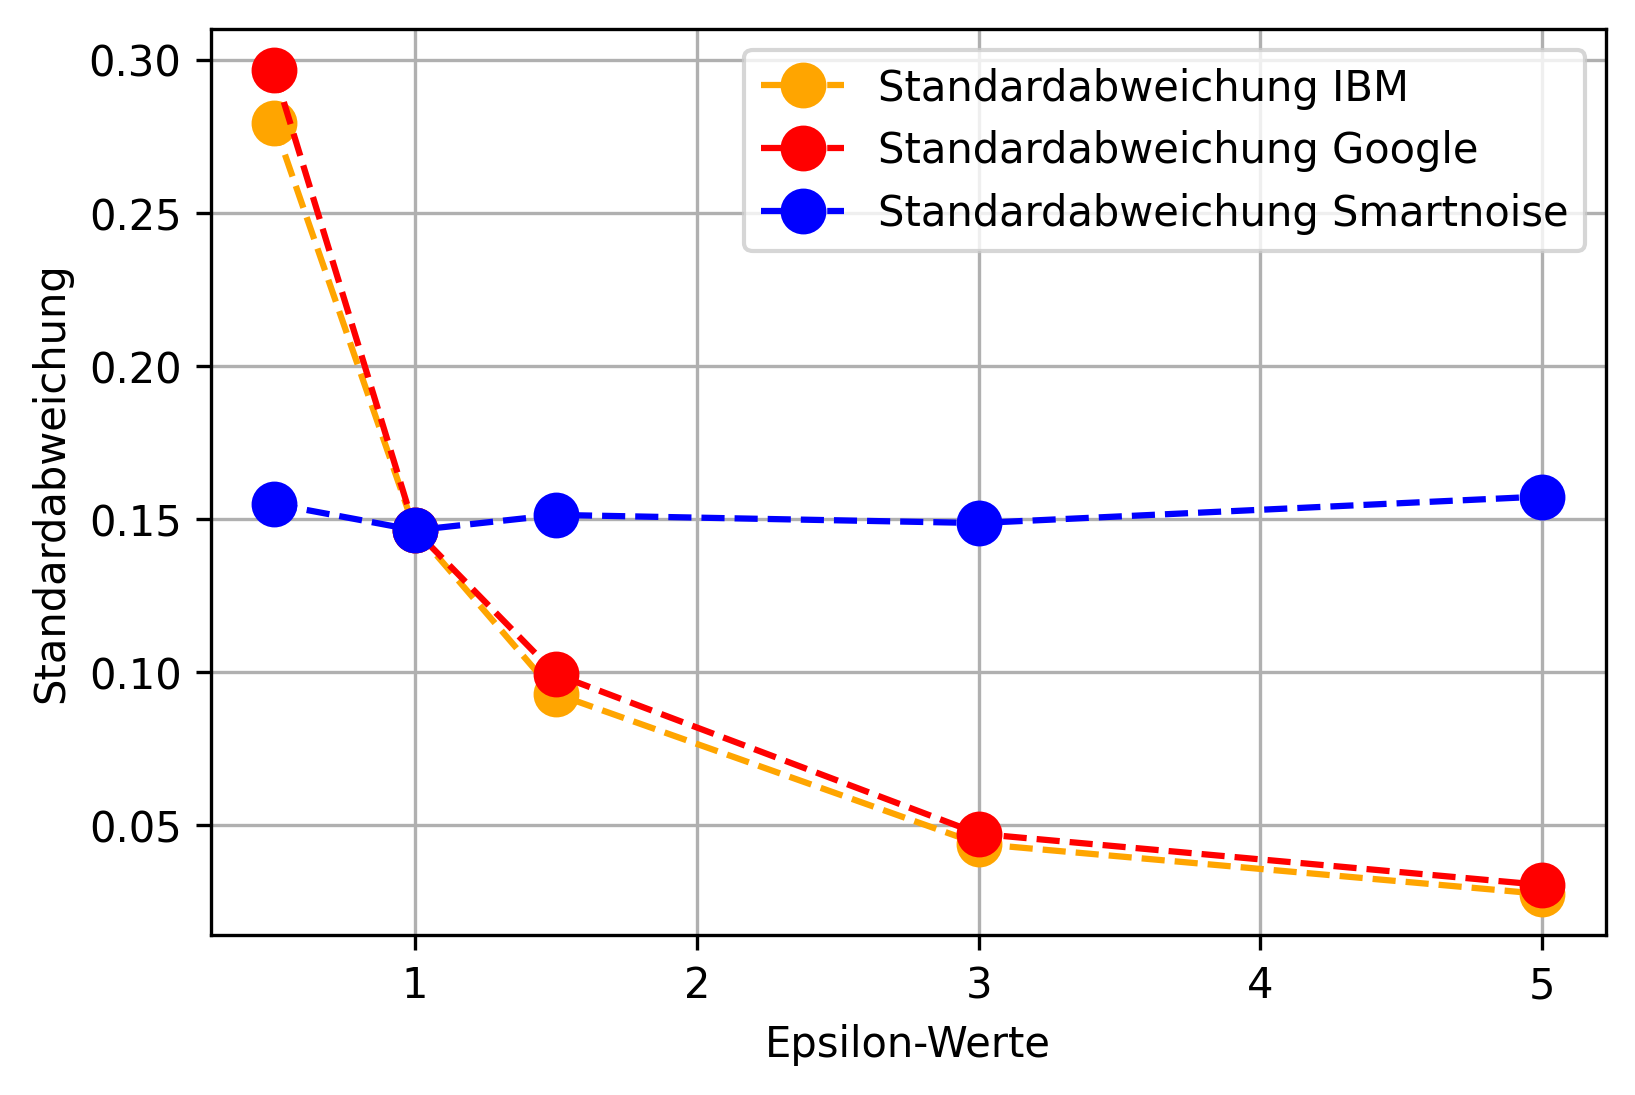
\includegraphics[scale=0.6]{./images/together_std.png}
	\caption{Die Gesamtübersicht der drei Frameworks in der Metrik Standardabweichung.}
	\label{fig:together_std}
\end{figure}

\textbf{Vergleich: }
Im Ergebnis zeichnen sich deutliche Muster wie in \cref{fig:together_std} ab. IBM \gls{dp} sowie Google \gls{dp} verlaufen nahe zu parallel, da beide mit steigendem $\epsilon$-Wert weniger Verrauschen zu den Daten hinzufügen. Die verrauschten Ausgaben weichen weniger ab, sodass die Genauigkeit zunimmt. Die minimale Genauigkeit ist am ersten Punkt und die maximale Genauigkeit am letzten Punkt vorhanden. In Kontrast dazu steht die Kurve von Smartnoise SDK. Sie stagniert über die verschiedenen $\epsilon$-Werte hinweg und verliert keineswegs an Genauigkeit. Der Mechanismus beim Smartnoise SDK hat eine konstante Abweichung in seiner verrauschten Ausgabe, weswegen die erwartete höhere Genauigkeit in den größeren $\epsilon$-Werten verloren geht. 

\newpage
\section{Erwartungstreue}
In diesem Abschnitt wird die Verzerrung der verrauschten Daten betrachtet. Inwieweit sie von den unveränderten Daten abweichen. Diese Auswirkungen betreffen die Semantik der Daten.
\subsection{Mittlere vorzeichenbehaftete Abweichung}
Mit dieser Metrik wird gefolgert, ob das Verrauschen die Semantik des unveränderten Datensatzes bewahrt und ob im Durchschnitt zu wenig oder zu viel hinzugerechnet wurde. Dafür war die Eingabe zum einen der erste verrauschte Datensatz und zum anderen der unveränderte Datensatz.
\begin{figure}[htbp]
	\centering
	\subfloat[Das Ergebnis von IBM \gls{dp} für die Standardabweichung.]{
		\label {fig:ibm_msd}
		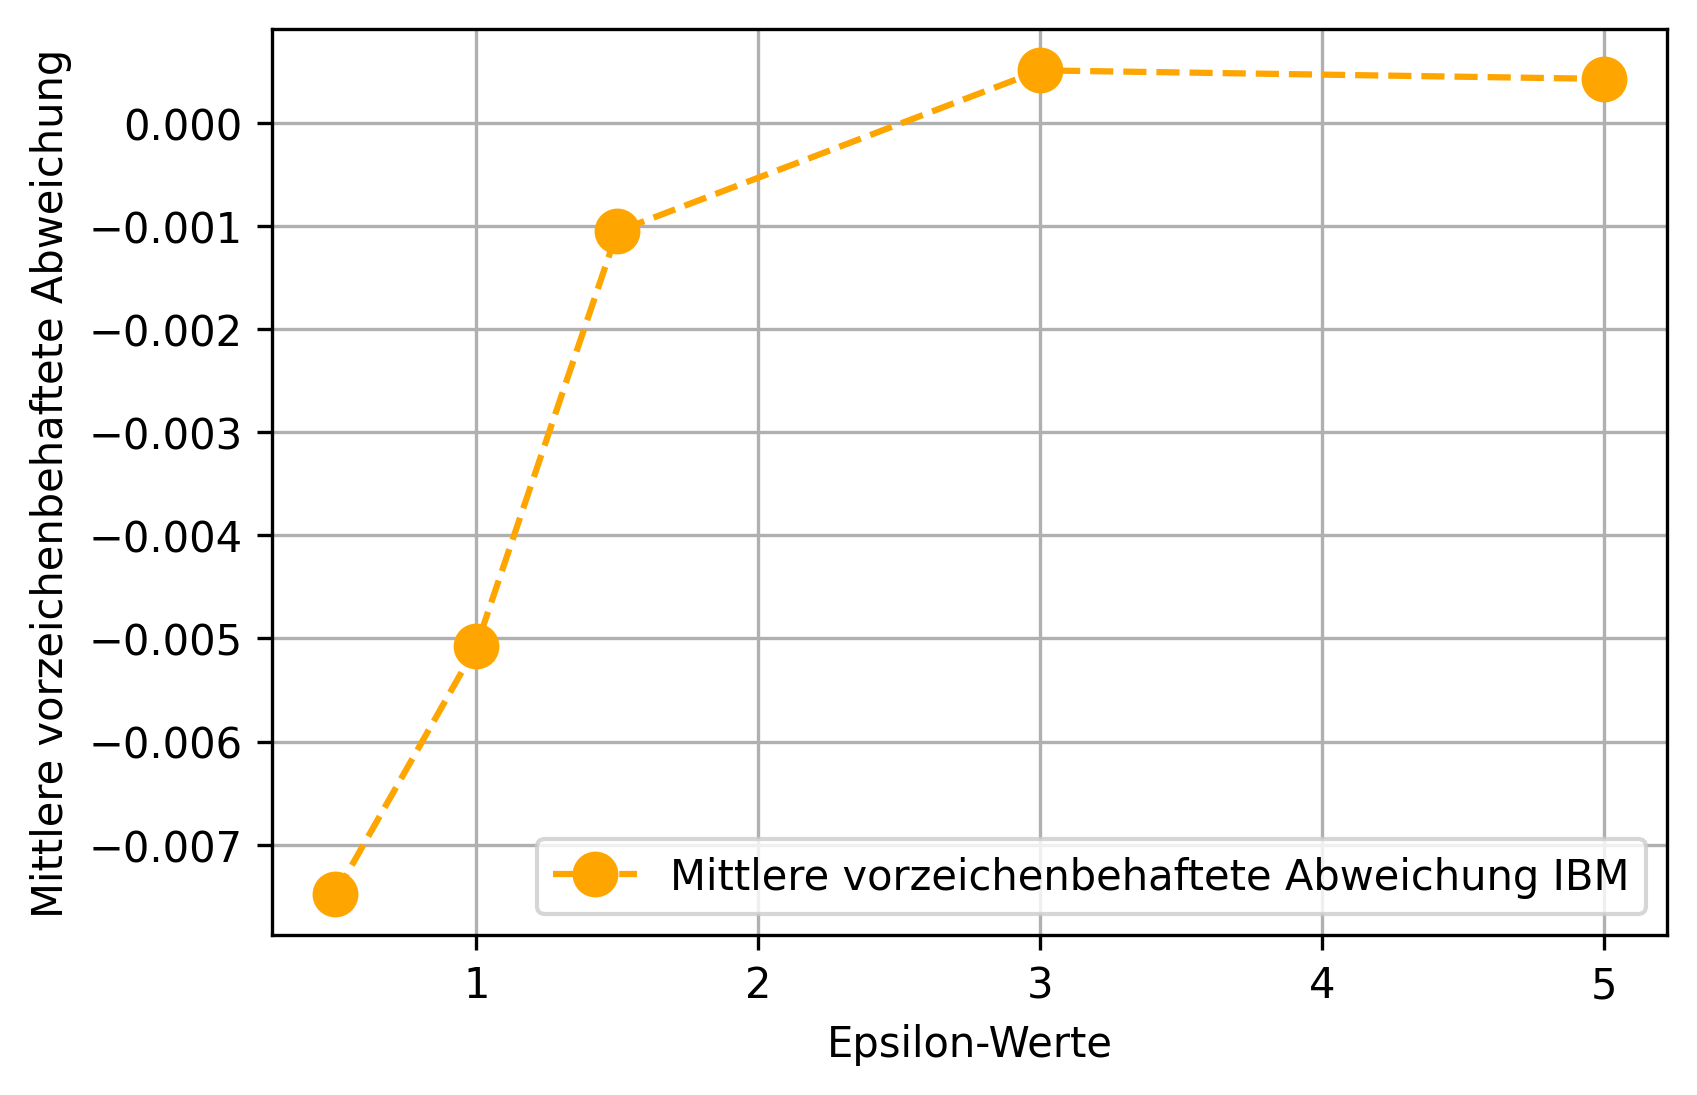
\includegraphics[scale=0.4]{./images/ibm_msd.png}
	} \qquad
	\subfloat[Das Ergebnis von Google für die Standardabweichung.]{
		\label {fig:google_msd}
		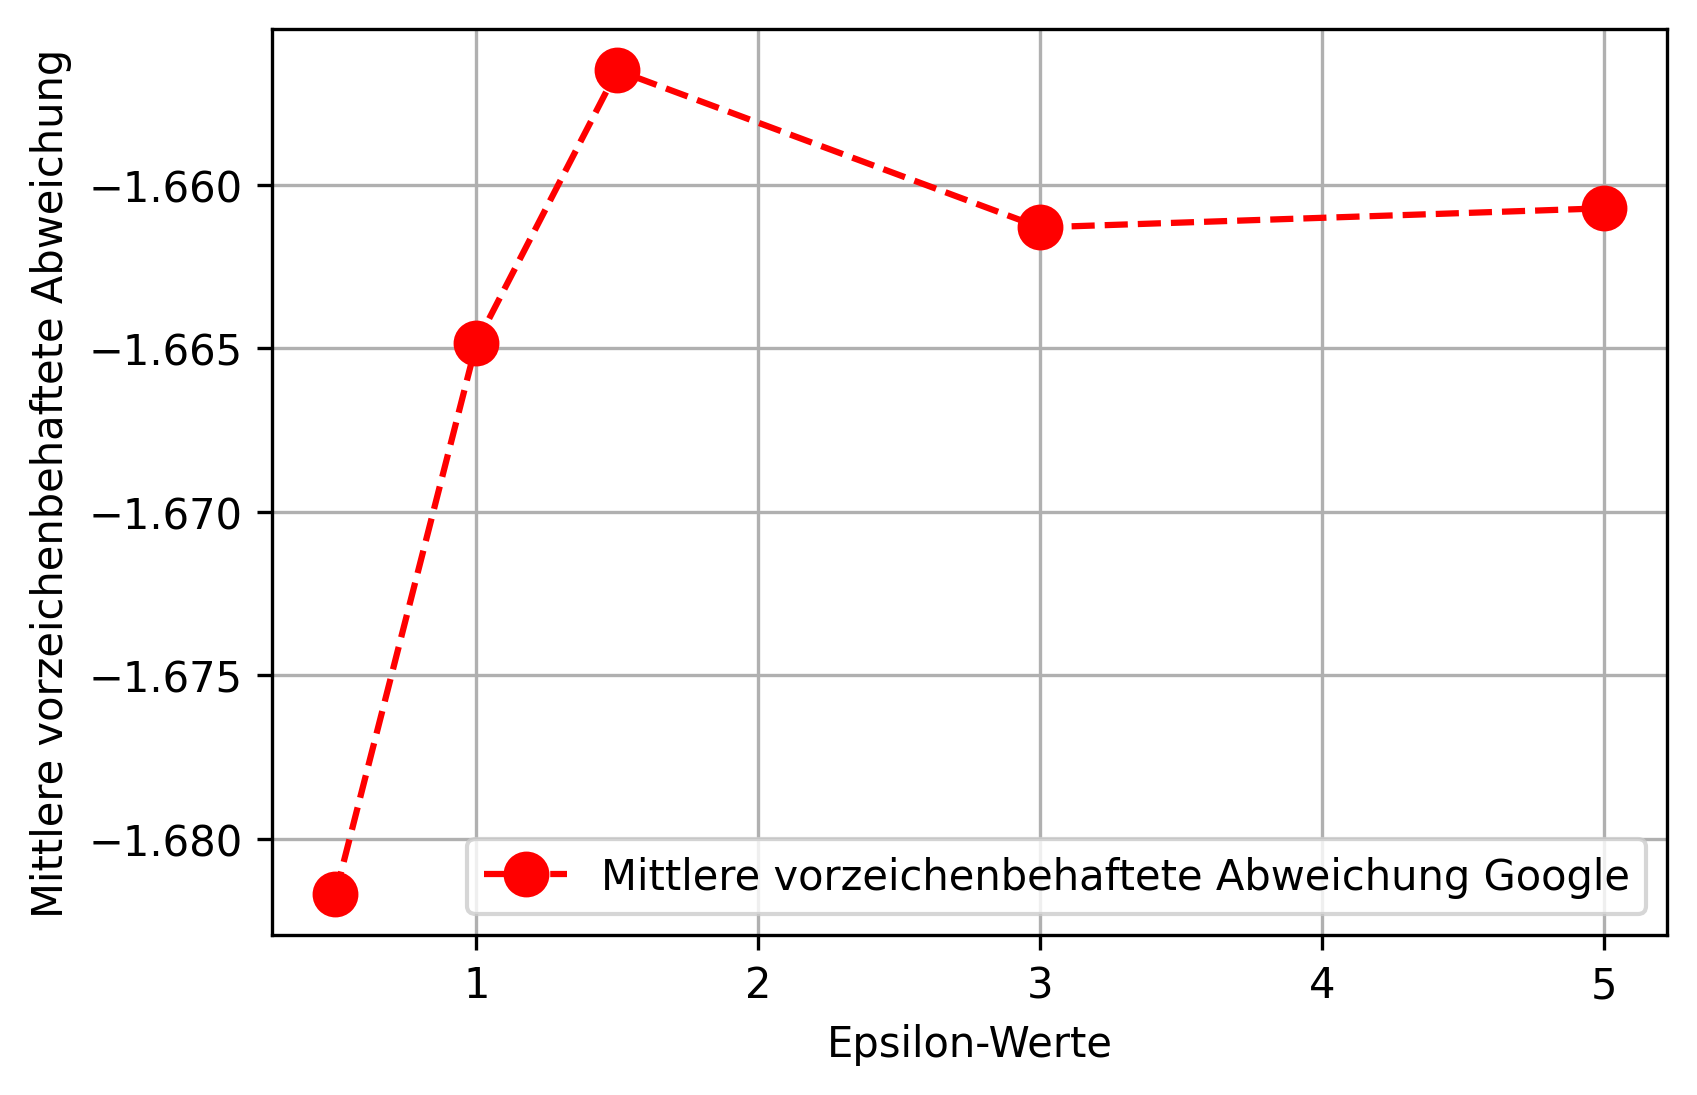
\includegraphics[scale=0.4]{./images/google_msd.png}
	}
	\subfloat[Das Ergebnis von Smartnoise SDK für die Standardabweichung.]{
		\label {fig:sn_msd}
		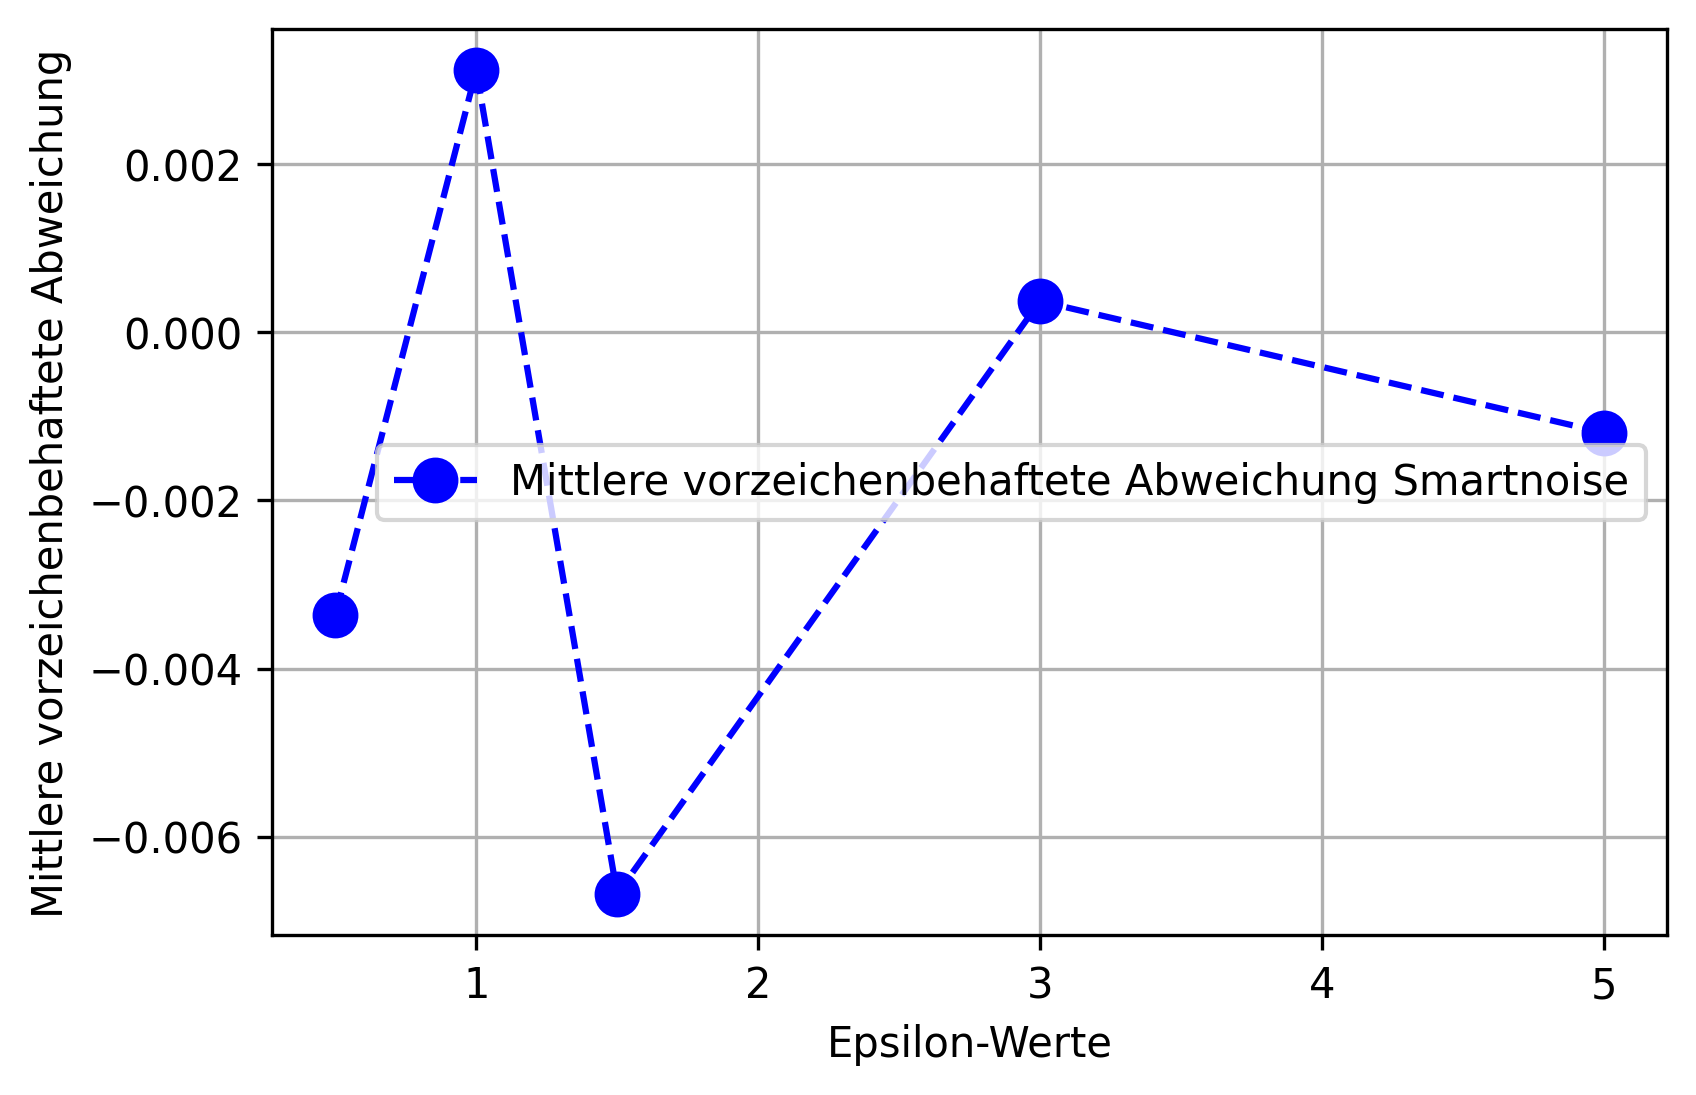
\includegraphics[scale=0.4]{./images/sn_msd.png}
	}
	\caption{Die Ergebnisse der Standardabweichung für die $\epsilon$-Werte [0,5;1,0;1,5;3,0;5,0] der drei Frameworks.}
	\label{fig:msd}
\end{figure}

\textbf{Erwartetes Ergebnis:}
Nach dem Laplace Mechanismus hat die Laplace Verteilung den Erwartungswert $\mu$=$0$. Dadurch soll die Aussagekraft der verrauschten Daten beibehalten werden. Bei kleinen $\epsilon$-Werten ist ein höherer Wert der Metrik zu erwarten,  da dann die Privatsphäre mehr geschützt wird und das Verrauschen verstärkt ist. Das Vorzeichen spielt in erster Rolle keine essentielle Rolle, sondern der Betrag des Wertes. Es kann insoweit ein typisches Verhalten des Mechanismus nach zeigen, ob grundsätzlich zu viel oder zu wenig hinzugefügt worden ist.

\textbf{IBM \gls{dp} Ergebnis:}
Die Kurve in \cref{fig:ibm_msd} verläuft mit steigendem $\epsilon$ streng monoton steigend gegen den Wert $0$, sodass die Verzerrung stets abnimmt. Die semantische Nutzbarkeit der Daten bleibt erhalten. Im Gesamtüberblick der Werte liegen sie bei fast $0$, wodurch ein Verlust der semantischen Aussagekraft  nicht einhergeht.

\textbf{Google Ergebnis:}
In den Zwischenergebnissen sinkt der Wert des Durchschnitts durch das Verrauschen des Mechanismus auf 34. In \cref{fig:google_msd} folgt die Konsequenz durch diese Metrik, welche sehr groß und ausschließlich negativ ausgefallen ist. Dies zeigt ein Muster des Mechanismus auf. Eine höhere Verzerrung liegt bei den ersten zwei Punkten wie erwartet vor, jedoch der dritte Punkt ist ein Ausreißer, wogegen die letzten zwei Punkte stagnieren. Die semantische Bedeutung ist bei den letzten zwei Punkten konstant gehalten, wogegen sie zu vor abnimmt. Insgesamt folgt bei der Auswertung ein hoher semantischer Verlust der verrauschten Daten, somit ebenfalls an Nutzbarkeit.

\textbf{Smartnoise SDK Ergebnis:}
Die Werte der Metrik liegen in \cref{fig:sn_msd} sehr nahe an $0$. Ein Verschwinden der semantischen Bedeutung der verrauschten Datensätze geht nicht hervor. Die Verteilung der Punkte in der Abbildung sind verstreut, sodass kein konstantes Verhalten des Mechanismus hervorgeht. Grundsätzlich gilt bei kleinen $\epsilon$-Werten betragsmäßig ein höherer Wert als bei großen, damit die Verzerrung die Nachvollziehbarkeit der unveränderten Daten erschwert (Schutz der Privatsphäre). Hier wird dies nicht eingehalten.
\begin{figure}[htbp]
	\centering
	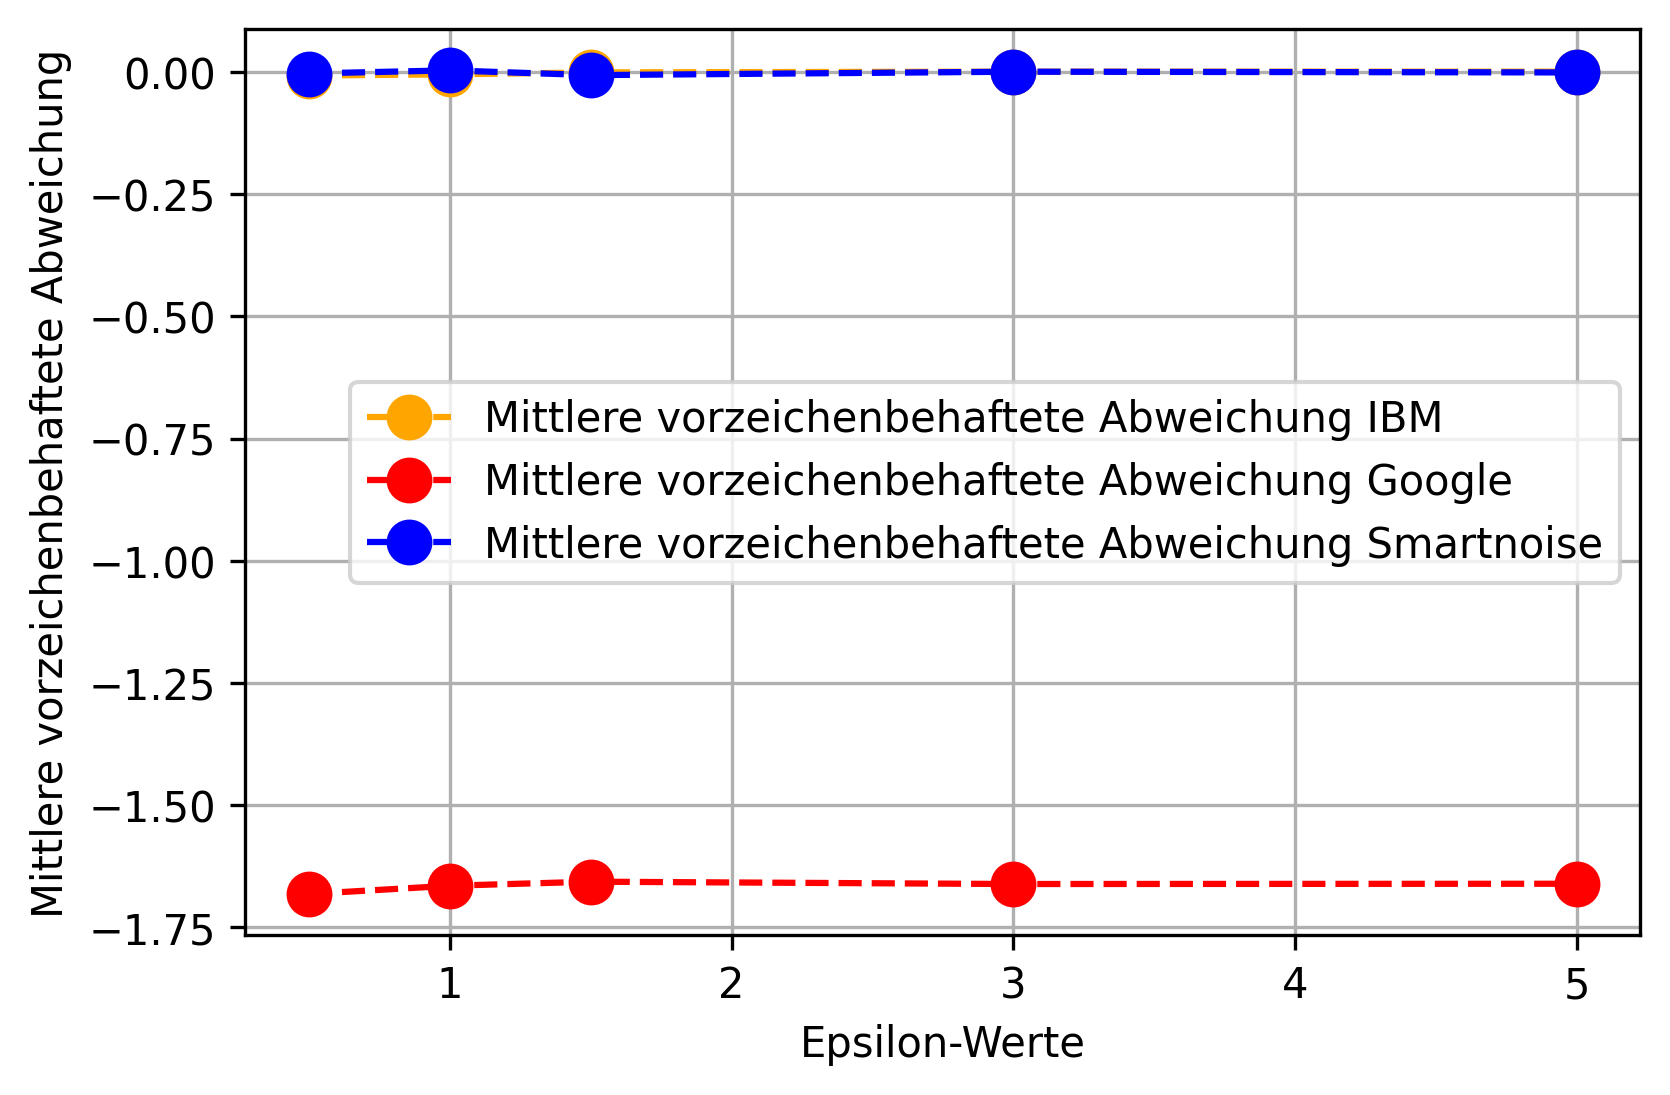
\includegraphics[scale=0.6]{./images/together_msd.png}
	\caption{Die Gesamtübersicht der drei Frameworks in der Metrik Mittlere vorzeichenbehaftete Abweichung.}
	\label{fig:together_msd}
\end{figure}

\textbf{Vergleich: }
Die beiden Frameworks Smartnoise SDK sowie IBM \gls{dp} bewahren die Nutzbarkeit der verrauschten Datensätze auf einem Niveau wie in \cref{fig:together_msd} erkennbar. Dies erlaubt den verrauschten Datensätze eine hohe Aussagekraft zu behalten. In Verhältnis dazu verzerrt Google durchschnittlich die Werte sehr durch zu viel negatives Rauschen. Damit geht ein großer Verlust der Semantik der Daten einher. In den Zwischenergebnissen liegen daher die verrauschten Werte bei den erstgenannten Frameworks bei ca. 36, wogegen bei Google stets um den Wert 34.
\newpage
\section{Performance}
In diesem Kapitel wird die Performance der Berechnung von verrauschten Werten evaluiert. Die Berechnung sind die 10,000 verrauschten Durchschnittswerte, die aus den 5 $\epsilon$-Werten mit jeweils 1,000 Durchführungen für zwei Datensätze resultieren. Die Anzahl an Iterationen für IBM \gls{dp} und Google \gls{dp} beträgt 1,000 und beim Smartnoise SDK 100.

\subsubsection{Bedingungen}
Zunächst erfolgt die Messung der Ausführungszeit ausschließlich der zuvor genannten Berechnung. Es werden keine Overheads wie die Verbindung, Einlesung oder Verarbeitung der Daten usw. berücksichtigt. Die Relevanz liegt auf der verrauschten Funktion durch das Framework.

Im Gegensatz dazu wurde Google \gls{dp} in der Programmiersprache Java genutzt. Eine Verlagerung der Berechnung auf den Server war aufgrund von serverseitigen Einstellungen zu aufwendig, weswegen sie lokal durchgeführt wurde. Trotz dessen ist dies nicht von belangen, denn die Ausführungszeit ist lokal sehr kurz. Somit wird hierbei schon ein Trend des Frameworks klar ersichtlich.

\subsubsection{Ausführungszeiten der Frameworks}
\begin{figure}[htbp]
	\centering
	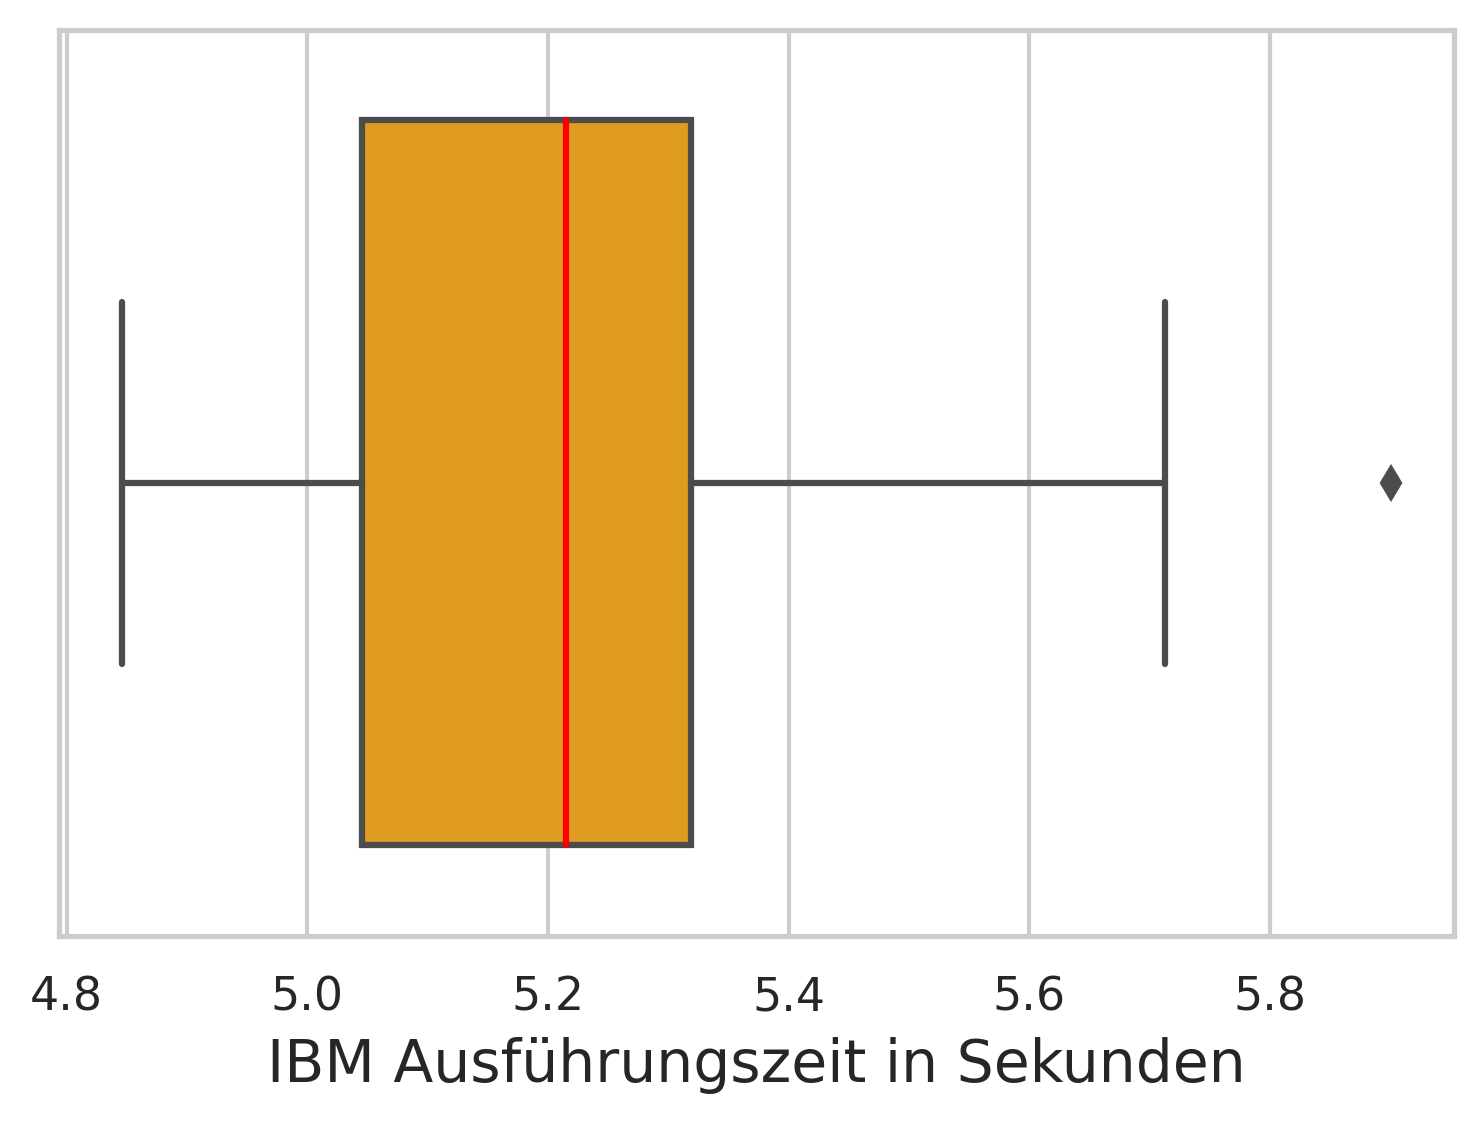
\includegraphics[scale=0.6]{./images/boxplot_ibm.png}
	\caption{Die Ausführungszeit von IBM \gls{dp} für die Berechnung der verrauschten Durchschnittswerte (10,000 Werte).}
	\label{fig:boxplot_ibm}
\end{figure}
\textbf{Ergebnis von IBM \gls{dp}:}
In \cref{fig:boxplot_ibm} ist der Boxplot der Ausführungszeiten von IBM \gls{dp} dargestellt. Der Median für die Zeit liegt bei 5,2 Sekunden. 50 \% der Iterationen weisen eine Zeit zwischen 5.05 und 5,32 Sekunden auf. Im unteren Viertel liegen die Werte zwischen 4.85 und 5.05 Sekunden und im oberen Viertel zwischen 5,32 und 5,71 Sekunden. Im Gesamten gibt es nur einen einzigen Ausreißer mit der Ausführungszeit 5,90. Insgesamt verläuft die Ausführungszeit schnell und stabil. Damit kann es mit hoher Nutzbarkeit angewendet werden.

\begin{figure}[htbp]
	\centering
	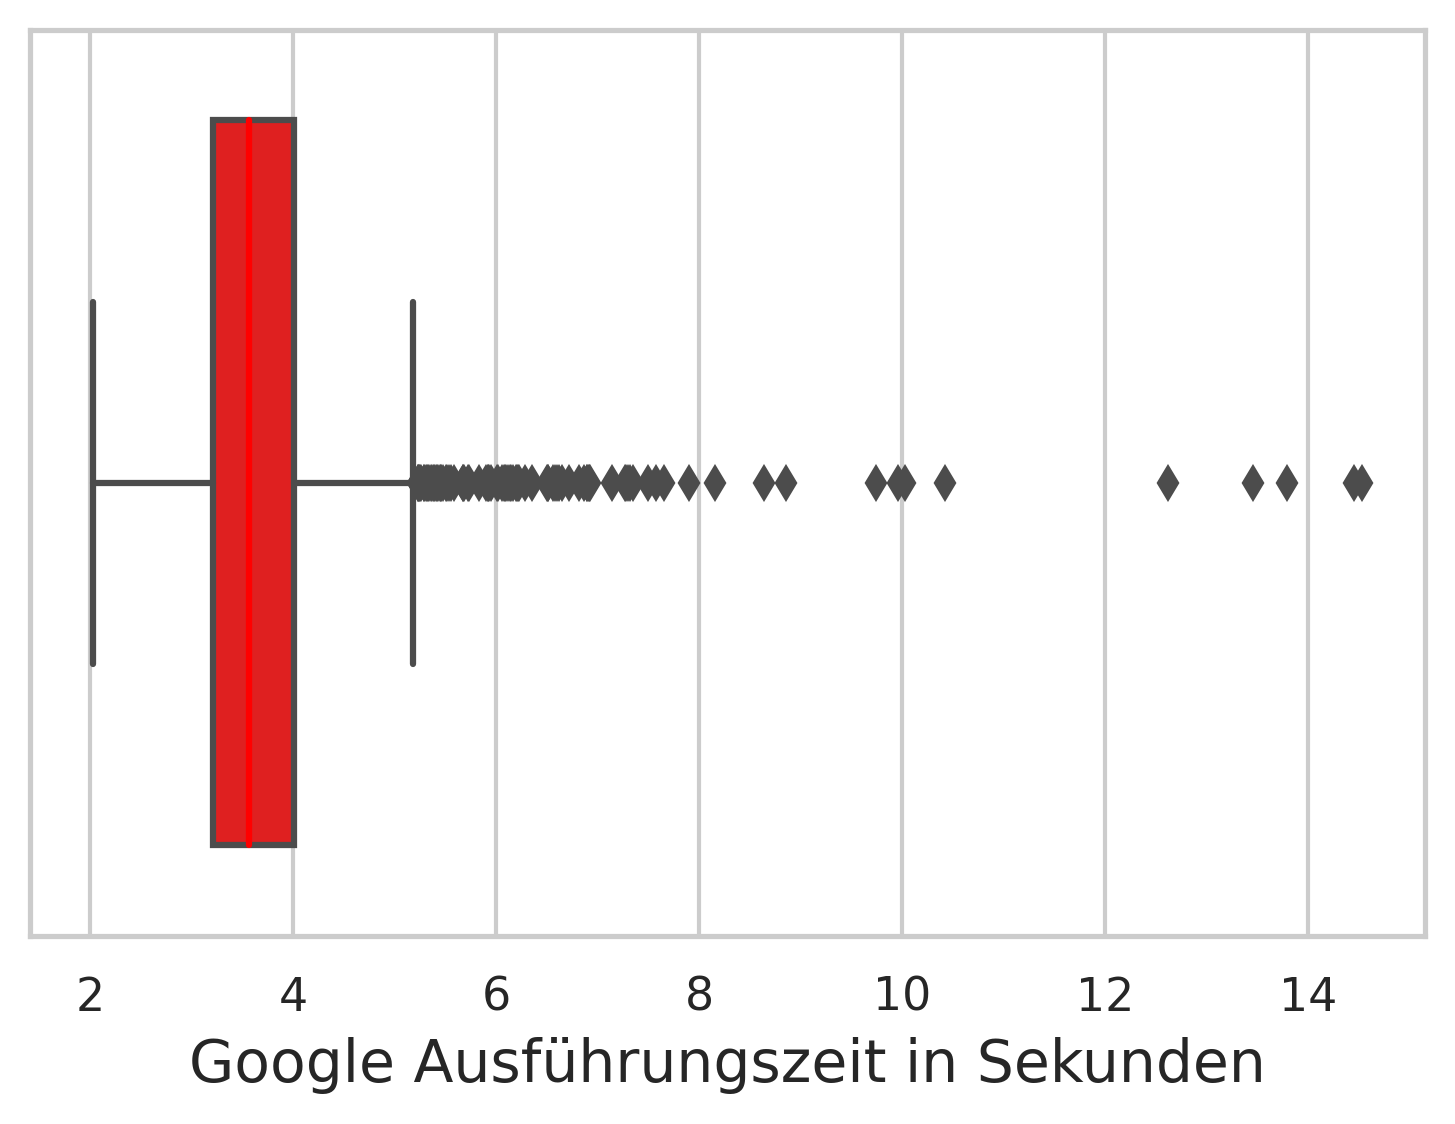
\includegraphics[scale=0.6]{./images/boxplot_google.png}
	\caption{Die Ausführungszeit von Google für die Berechnung der verrauschten Durchschnittswerte (10,000 Werte).}
	\label{fig:boxplot_google}
\end{figure}

\textbf{Ergebnis von Google:}
In \cref{fig:boxplot_google} ist der Boxplot der Ausführungszeiten von Google dargestellt. Der Median liegt bei 3,6 Sekunden, welcher eine schnelle Ausführungszeit aufzeigt. 50 \% der Iterationen weisen eine Zeit zwischen 3,21 und 4,01 Sekunden auf. Im unteren Viertel liegen die Werte zwischen 2,03 und 3,21 Sekunden und im oberen Viertel zwischen 4,01 und 5,18 Sekunden. Die Anzahl an Ausreißer beträgt 93 und betrifft 9,3 \% der Ausführungen. Dies weist eine gewisse Instabilität auf, die jeden 10. Durchlauf betrifft. Hierbei liegt das Maximum bei 14,53 Sekunden, wobei einige Ausreißer wie 14,45 Sekunden, 13,79 Sekunden und 12,62 Sekunden in die Nähe dessen liegen. Das Minimum liegt bei 2,03 und weißt unterdessen keine Ausreißer auf. Die Ursache für das vermehrte Auftreten von Ausreißern ist nicht erklärbar und auf das Framework zurückzuführen.

\textbf{Ergebnis von Smartnoise SDK:}
Bei Smartnoise SDK beansprucht die Ausführungszeit ca. 2 Stunden, weswegen eine Evaluation von 1000 Iterationen im Rahmen der Arbeit nicht umsetzbar gewesen ist. Aufgrund dessen beträgt die Anzahl für die Iteration 100, trotz dessen ein klares Muster der Laufzeit sich abzeichnet.

In \cref{fig:boxplot_sn} wird die lange Ausführungszeit deutlich. Der Median liegt hierbei bei 1,98 Stunden, also fast 2 Stunden. Ca. 25 \% der Ausführungszeiten liegen über 2 Stunden. Die Spanne dabei beträgt zwischen 2,03 und 2,19 Stunden. Der untere Quantil umfasst die Werte zwischen 1,75 und 1,89 Stunden. Insgesamt sind keine Ausreißer vorgekommen.
\begin{figure}[p]
	\centering
	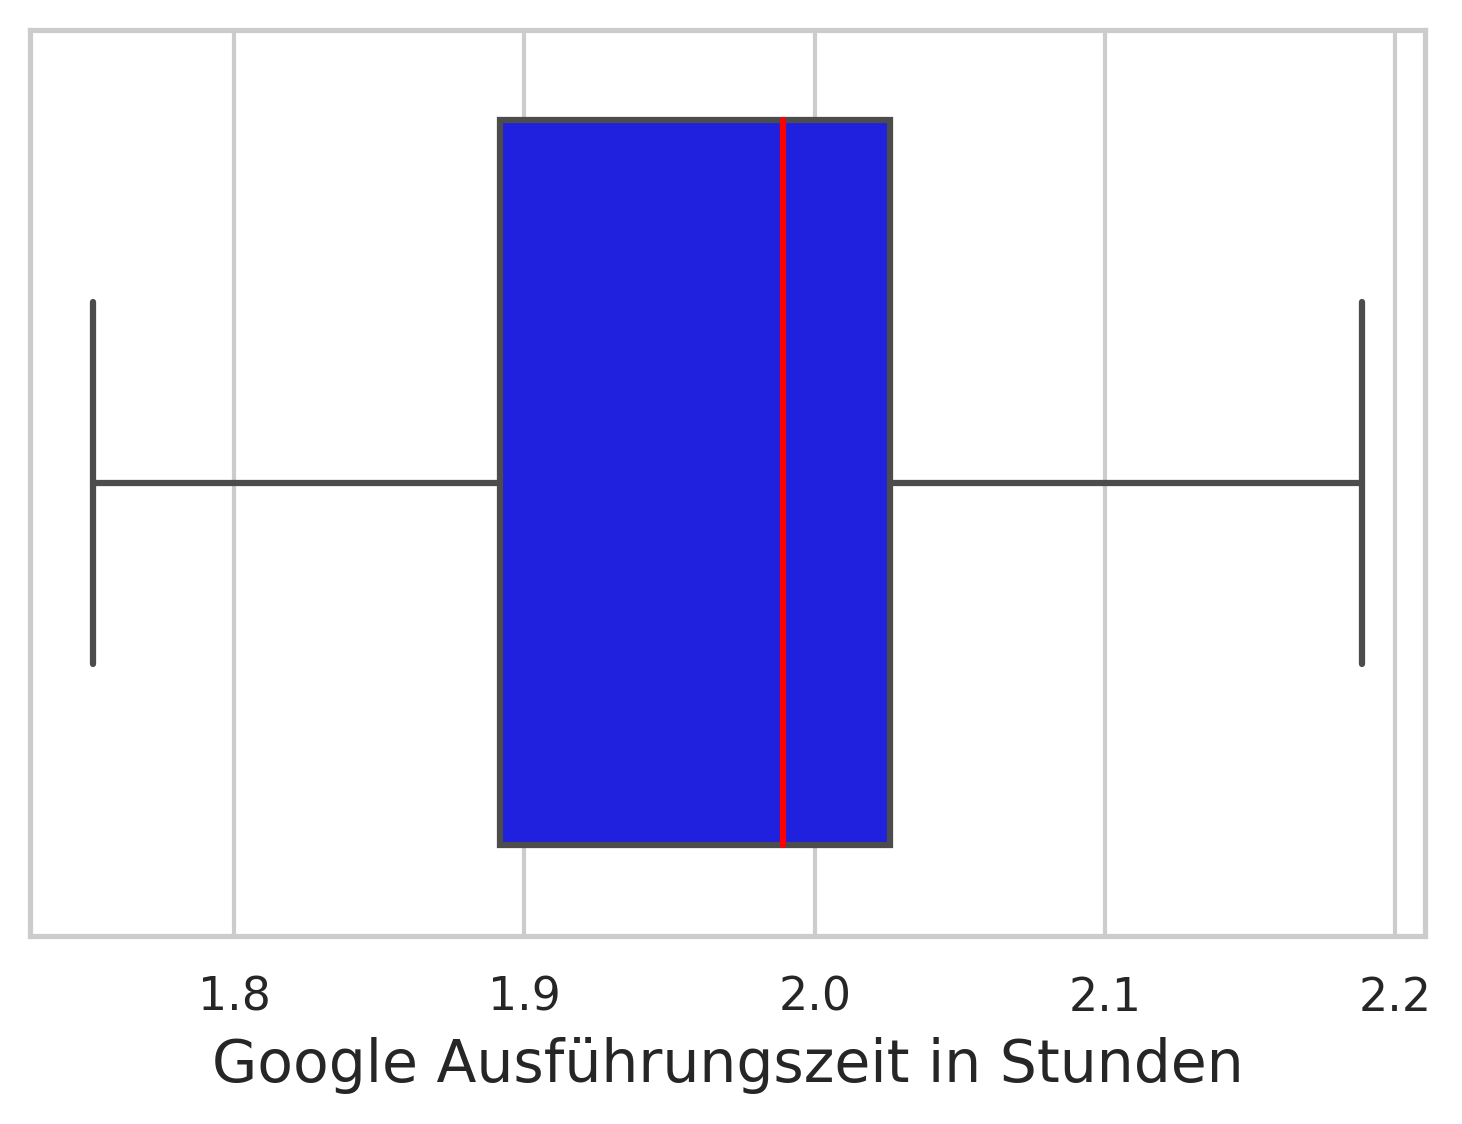
\includegraphics[scale=0.6]{./images/boxplot_sn.png}
	\caption{Die Ausführungszeit von Smartnoise SDK für die Berechnung der verrauschten Durchschnittswerte (10,000 Werte).}
	\label{fig:boxplot_sn}
	\vspace{100in}
\end{figure}